\documentclass{book}
\usepackage[fleqn]{amsmath}
\usepackage{graphicx}
\usepackage{mathrsfs}
\usepackage{color}
\usepackage{amssymb}
\usepackage{amsfonts,amssymb}
\usepackage{algorithm}
\usepackage{algorithmic}
\usepackage{array}
\usepackage{latexsym}
\usepackage{tabularx}
\usepackage{dsfont}
\usepackage{subfigure}

\usepackage{tabularx} % extra features for tabular environment
\usepackage{amsmath}  % improve math presentation
\usepackage{graphicx} % takes care of graphic including machinery
\usepackage{bm}
\usepackage{bbold} % support \mathbbm{1}
\usepackage{mathrsfs}
\usepackage{enumerate}
\usepackage{amsthm,amsmath,amssymb}
\usepackage[margin=1in,letterpaper]{geometry} % decreases margins
\usepackage{cite} % takes care of citations
\usepackage[final]{hyperref} % adds hyper links inside the generated pdf file

\newcommand{\NN}{\mathbb{N}}
\newcommand{\RR}{\mathbb{R}}
\newcommand{\FF}{\mathbb{F}}
\newcommand{\cA}{\mathcal{A}}
\newcommand{\cB}{\mathcal{B}}
\newcommand{\cC}{\mathcal{C}}
\newcommand{\cD}{\mathcal{D}}
\newcommand{\cE}{\mathcal{E}}
\newcommand{\cF}{\mathcal{F}}
\newcommand{\cG}{\mathcal{G}}
\newcommand{\cH}{\mathcal{H}}
\newcommand{\cI}{\mathcal{I}}
\newcommand{\cR}{\mathcal{R}}
\newcommand{\cS}{\mathcal{S}}
\newcommand{\cN}{\mathcal{N}}
\newcommand{\EE}[1]{\mathbb{E} \left[#1\right]}
\newcommand{\PP}[1]{\mathbb{P} \left(#1\right)}

\newcommand{\bP}{\mathbb{P}}
\newcommand{\bQ}{\mathbb{Q}}


\newcommand{\abs}[1]{\left| #1 \right|}
\newcommand{\bracket}[1]{\left(#1\right)}
\newcommand{\norm}[1]{\left\| #1 \right\|}
\newcommand{\set}[1]{\left\{ #1 \right\}}
\newcommand{\Angle}[1]{\langle #1 \rangle}

\newcommand{\bOne}[1]{\mathds{1} \! \left\{#1\right\}}
\DeclareMathOperator*{\argmax}{argmax}
\DeclareMathOperator*{\argmin}{argmin}

\newtheorem{theorem}{Theorem}
\newtheorem{lemma}{Lemma}
\newtheorem{definition}{Definition}
\newtheorem{proposition}{Proposition}

\hypersetup{
	colorlinks=true,       % false: boxed links; true: colored links
	linkcolor=blue,        % color of internal links
	citecolor=blue,        % color of links to bibliography
	filecolor=magenta,     % color of file links
	urlcolor=blue
}
\usepackage{blindtext}


\title{Solutions}
\author{}
\date{}

\begin{document}
\maketitle

%!TEX root =  main.tex

% for theorem etc ************************************************
% \newtheorem{theorem}{Theorem}[section]
% \newtheorem{lemma}[theorem]{Lemma}
% \newtheorem{proposition}[theorem]{Proposition}
% \newtheorem{corollary}[theorem]{Corollary}
% \newtheorem{definition}{Definition}[section]
% \newtheorem{remark}{Remark}[section]
% \newtheorem{example}{Example}[section]
% \newenvironment{solution}{\begin{proof}[Solution]}{\end{proof}
% ************************************************

\chapter*{Chapter 2 Foundations of Probability}
\label{sec:second}

% \kant[7-11] % Dummy text

% \begin{theorem}[{\cite[95]{AM69}}]
%     \label{thm:dedekind}
%     Let \( A \) be a Noetherian domain of dimension one. Then the following are equivalent:
%     \begin{enumerate}
%         \item \( A \) is integrally closed;
%         \item Every primary ideal in \( A \) is a prime power;
%         \item Every local ring \( A_\mathfrak{p} \) \( (\mathfrak{p} \neq 0) \) is a discrete valuation ring.
%     \end{enumerate}
% \end{theorem}

\noindent\textbf{2.1} (\textsc{Composing random elements}) Show that if $f$ is $\mathcal{F}/\mathcal{G}$-measurable and $g$
is $\mathcal{G}/\mathcal{H}$-measurable for sigma algebras $\mathcal{F}$,$\mathcal{G}$ and $\mathcal{H}$ over appropriate spaces, then
their composition, $g \circ f$ (defined the usual way: $( g \circ f )(\omega) = g(f(\omega)), \omega \in \Omega)$, is
$\mathcal{F}/\mathcal{H}$-measurable.

\begin{proof}
    Since $g$ is $\mathcal{G}/\mathcal{H}$-measurable, therefore $\forall C \in \mathcal{H}$,\ $ \exists  B=g^{-1}(C)\in \mathcal{G} $ . Similarly, since $f$ is $\mathcal{F}/\mathcal{G}$-measurable, $\forall B \in \mathcal{G}$,\ $ \exists  A=f^{-1}(B)\in \mathcal{F} $ . Thus $\forall C \in \mathcal{H}$, \ $ \exists  A=f^{-1}(g^{-1}(C))=(g\circ f)^{-1}(C)\in \mathcal{F} $ and the proof is complete. \\

\end{proof}

% \subsubsection{}

\noindent\textbf{2.2}
Let $X_1,\dots,X_n$ be random variables on $(\Omega, \mathcal{F})$. Prove that $X=( X_1 ,\dots,X_n )$ is a random vector.
\begin{proof}
    Since $X_i$ is a random variable ($\forall i=1,2,...,n$), it holds that $X_i$ is $\cF/\cB(\RR)$-measurable, which means that $\forall B \in \cB(\RR)$, $X_i^{-1}(B) \in \cF$.
    We first prove that $X$ is $\cF/(\cB(\RR) \times \cB(\RR)\times\cdots \cB(\RR) )$-measurable (totally $n$ $\cB(\RR)$s). $\forall A=A_1\times A_2 \times \cdots \times A_n  \in \cB(\RR) \times \cB(\RR)\times\cdots \cB(\RR)$, $X^{-1}(A) =X_1^{-1}(A_1) \cap X_2^{-1}(A_2) \cap \cdots \cap X_n^{-1}(A_n) \in \cF$, which holds since $X_i^{-1}(A_i) \in \cF, \forall i =1,2,...,n$ and $\cF$ is a $\sigma$-algebra. Thus we conclude that $X$ is $\cF/(\cB(\RR) \times \cB(\RR)\times\cdots \cB(\RR) )$-measurable.

    By definition $\cB(\RR^n) = \sigma (\cB(\RR) \times \cB(\RR)\times\cdots \cB(\RR))$ (totally $n$ $\cB(\RR)$s). And according to the property in 2.5(b), we can get that $X$ is $\mathcal{F}/\mathcal{B}(\RR^n)$-measurable, thus it is a random vector.\\
    % We claim that $X=(X_1,X_2,...,X_n)$ is $\mathcal{F}/\mathcal{B}(\mathbb{R}^n)$ measurable. Define $a=(a_1,a_2,...,a_n)$ $b=(b_1,b_2,...,b_n)$ with $a,b\in \mathbb{R}^n$ where $a<b$. Since $X_1,X_2,...,X_n$ is $\mathcal{F}/\mathcal{B}(\mathbb{R})$ measurable, therefore $\exists A_1=X^{-1}_1((a_1,b_1)),A_2=X^{-1}_2((a_2,b_2)),...,A_n=X^{-1}_n((a_n,b_n))\in \mathcal{F}$. Let $A=A_1\cap A_2 \cap...\cap A_n=\bigcap\limits^{n}_{i=1}A_i$. It follows that $X^{-1}((a,b))=\bigcap\limits^{n}_{i=1}((a,b))=A\in \mathcal{F}$. Therefore $X$ is $\mathcal{F}/\mathcal{B}(\mathbb{R}^n)$ measurable and $X$ is random vector. \\
\end{proof}

% \subsubsection{}

\noindent\textbf{2.3}
(\textsc{Random variable induced $\sigma$-algebra}) Let $\mathcal{U}$ be an arbitrary set and
$( \mathcal{V}, \Sigma)$ a measurable space and $X : \mathcal{U} \rightarrow \mathcal{V}$ an arbitrary function. Show that
$\Sigma_X = \{X ^{-1} (A) : A \in \Sigma\}$ is a $\sigma$-algebra over $\mathcal{U}$.

\begin{proof}
    \begin{enumerate}
        \item[(i)] We need to show that $\Sigma_X$ is closed under countable union. Let $U_i=X^{-1}(A_i),A_i\in \Sigma, i\in \mathbb{N}$. It follows that $\bigcup\limits^{\infty}_{i=1}U_i=\bigcup\limits^{\infty}_{i=1}X^{-1}(A_i)=X^{-1}(\bigcup\limits^{\infty}_{i=1}A_i)$. Since $\bigcup\limits^{\infty}_{i=1}A_i\in \Sigma$, $\bigcup\limits^{\infty}_{i=1}U_i\in \Sigma_X$.
        \item[(ii)] We need to show that $\Sigma_X$ is closed under set subtraction $-$. $\forall U_1,U_2\in \Sigma_X$,$U_1-U_2=X^{-1}(A_1)-X^{-1}(A_2)=X^{-1}(A_1-A_2)$. Since $A_1-A_2\in \Sigma$, $U_1-U_2\in \Sigma_X$.
        \item[(iii)] We need to show that $\Sigma_X$ is closed to $\mathcal{U}$ itself. Since $\mathcal{U}=X^{-1}(\mathcal{V})$ and $\mathcal{V}\in \Sigma$, it follows that $\mathcal{U}\in \Sigma_X$.
        \end{enumerate}
\end{proof}



\noindent\textbf{2.4}
Let $(\Omega,\mathcal{F})$ be a measurable space and $A \subseteq \Omega$ and $\mathcal{F}_{|A} = \{A \cap B: B \in \mathcal{F}\}$.

\begin{proof}
    \begin{enumerate}
        \item[(a)] \begin{enumerate}
                \item[(i)] We need to show that $\mathcal{F}|_A$ is closed under countable union. Let $X_1=A\cap B_1,X_2=A\cap B_2,...$ and $X^{\prime}=\bigcup\limits^{\infty}_{i=1}X_i$ and $B^{\prime}=\bigcup\limits^{\infty}_{i=1}B_i$ where $B_1,B_2,...\in \mathcal{F}$. Since $\mathcal{F}$ is sigma algebra, $B^{\prime}\in \mathcal{F}$. Furthermore, since $X^{\prime}=\bigcup^{\infty}_{i=1}X_i=\bigcup^{\infty}_{i=1}A\bigcap B_i=A\bigcap\left(\bigcup\limits^{\infty}_{i=1}B_i \right)=A\bigcap B^{\prime}$, we can see that $X^{\prime}\in \mathcal{F}|_A$.
                \item[(ii)] We need to show that $\mathcal{F}|_A$ is closed under set subtraction $-$. $\forall X_1,X_2\in \mathcal{F}|_A$, $X_1-X_2=(A\bigcap B_1)-(A\bigcap B_2)=A\bigcap(B_1-B_2)$. Since $B_1-B_2\in \mathcal{F}$, it follows that $X_1-X_2\in \mathcal{F}|_A$.
                \item[(iii)] We need to show that $\mathcal{F}|_A$ is closed to $A$ itself. Since $\varnothing \in \mathcal{F}$, we have $\varnothing=A\bigcap\varnothing\in \mathcal{F}|_A$ and $A=\varnothing^{C}\in \mathcal{F}|_A$.
              \end{enumerate}
        \item[(b)] Let $P=\{ A\bigcap B:B\in \mathcal{F} \}, Q=\{ B: B\subset A, B\in \mathcal{F} \}$.
                \begin{enumerate}
                    \item[(i)] We claim that $P\subset Q$. Let $X=A\bigcap B, B\in \mathcal{F}$. Since $A\in \mathcal{F}$, $X=A\bigcap B\in \mathcal{F}$. Furthermore, $X\in Q=\{B:B\subset A, B\in \mathcal{F} \}$.
                    \item[(ii)] We claim that $Q\subset P$. $\forall X\in Q$, we have $X\subset A$ and $X\in \mathcal{F}$, which means that $X=X\bigcap A$ and $X\in \mathcal{F}$. It follows that $X\in P$.
                    \item[(iii)] Take both (i)(ii) into consideration, we can see that $P=Q$.
                \end{enumerate}
        \end{enumerate}
\end{proof}


\noindent\textbf{2.5}
Let $\mathcal{G}\subseteq 2^{\Omega}$ be a non-empty collection of sets and define $\sigma(\mathcal{G})$ as the smallest
$\sigma$-algebra that contains $\mathcal{G}$. By `smallest' we mean that $\mathcal{F}\in 2^{\Omega}$ is smaller than
$\mathcal{F}^{\prime}\in 2^{\Omega}$ if $\mathcal{F}\subset \mathcal{F}^{\prime}$.
\begin{enumerate}
    \item[(a)] Show that $\sigma(\mathcal{G})$ exists and contains exactly those sets $A$ that are in every
    $\sigma$-algebra that contains $\mathcal{G}$.
    \item[(b)] Suppose $(\Omega^{\prime},\mathcal{F})$ is a measurable space and $X:\Omega^{\prime}\rightarrow \Omega$ be $\mathcal{F}/\mathcal{G}$-measurable. Show that X is also $\mathcal{F}/\sigma(\mathcal{G})$-measurable. (We often use this result to simplify the job of checking whether a random variable satisfies some measurability property).
    \item[(c)] Prove that if $A\in \mathcal{F}$ where $\mathcal{F}$ is a $\sigma$-algebra, then $\mathbb{I}\{A\}$ is $\mathcal{F}$-measurable.
\end{enumerate}

\begin{proof}
\begin{enumerate}
    \item[(a)] Let $\mathcal{K} = \{\mathcal{F} | \mathcal{F} \mbox{ is a }\sigma\mbox{-algebra and contains } \mathcal{G}\}$, It holds obviously that $\mathcal{K}$ is not an empty set since it contains $2^{\cG}$.

    Then $\bigcap_{\mathcal{F} \in \mathcal{K}}\mathcal{F}$ contains exactly those sets that are in every $\sigma$-algebra that contains $\mathcal{G}$. Given its existence, we only need to prove that $\bigcap_{\mathcal{F} \in \mathcal{K}}\mathcal{F}$ is the smallest $\sigma$-algebra that contains $\mathcal{G}$.

    First we show $\bigcap_{\mathcal{F} \in \mathcal{K}}\mathcal{F}$ is a $\sigma$-algebra. Since $\mathcal{F}$ is a $\sigma$-algebra and therefore $\Omega \in \mathcal{F}$ for all $\mathcal{F} \in \mathcal{K}$, it follows that $\Omega \in \bigcap_{\mathcal{F} \in \mathcal{K}}\mathcal{F}$. Next, for any $A \in \bigcap_{\mathcal{F} \in \mathcal{K}}\mathcal{F}$, $A^c \in \mathcal{F}$ for all $\mathcal{F} \in \mathcal{K}$. Since they are all $\sigma$-algebras, $A^c \in \mathcal{F}$ for all $\mathcal{F} \in \mathcal{K}$. Hence $A^c \in \bigcap_{\mathcal{F} \in \mathcal{K}}\mathcal{F}$. Finally, for any $\{A_i\}_i \subset \bigcap_{\mathcal{F} \in \mathcal{K}}\mathcal{F}$, $\{A_i\}_i \subset \mathcal{F}$ for all $\mathcal{F} \in \mathcal{K}$. Since they are all $\sigma$-algebras, $\bigcup_i A_i \in \mathcal{F}$ for all $\mathcal{F} \in \mathcal{K}$. Hence $\bigcup_i A_i \in \bigcap_{\mathcal{F} \in \mathcal{K}}\mathcal{F}$. 

    Next we want to prove $\bigcap_{\mathcal{F} \in \mathcal{K}}\mathcal{F}$ is the smallest $\sigma$-algebra that contains $\cG$. It is quite obvious that $\bigcap_{\mathcal{F} \in \mathcal{K}}\mathcal{F} \subseteq \mathcal{F}'$ for all $\mathcal{F}' \in \mathcal{K}$. 

    Above all, we have $\sigma(\cG)=\bigcap_{\mathcal{F} \in \mathcal{K}}\mathcal{F}$.

    \item[(b)] Define $\mathcal{H}=\left\{A: X^{-1}(A) \in \mathcal{F}\right\}$.
    To show $X$ is $\cF/\sigma(\cG)$-measurable, it is sufficient to prove $\sigma(\mathcal{G}) \subseteq \mathcal{H}$.

    First we prove that $\mathcal{H}$ is a $\sigma$-algebra.
    It holds that $\Omega \in \mathcal{H}$ since $X^{-1}(\Omega) = \Omega' \in \cF$.
    For any $A \in \mathcal{H}$, we have $X^{-1}(A) \in \mathcal{F}$, thus $X^{-1}(A^c) = X^{-1}(A)^c \in \mathcal{F}$, which holds since $\cF$ is a $\sigma$-algebra. Thus $A^c \in \mathcal{H}$. For any $A_i \in \cF$, $i=1,2,...$, $X^{-1}(A_i) \in \mathcal{F}$, $X^{-1}(\cup_i A_i) = \cup_i X^{-1}(A_i) \in \mathcal{F}$. We can then conclude $\cup_i A_i \in \cH$ and $\cH$ is a $\sigma$-algebra.


    Also, since $X$ is $\cF/\cG$-measurable, we have $\mathcal{G} \subseteq \mathcal{H}$.
    Thus $\mathcal{H}$ is $\sigma$-algebra that contains $\mathcal{G}$.
    By applying the result of (a), we have $\sigma(\mathcal{G}) \subseteq \mathcal{H}$, which completes the proof.

    \item[(c)] The idea is to show $\forall B \in \mathfrak{B}(\mathbb{R})$, $\mathbb{I}\{A\}^{-1}(B) \in \mathcal{F}$.

    If $\{0,1\} \in B$, $\mathbb{I}\{A\}^{-1}(B)=\Omega \in \mathcal{F}$. If $\{0\} \in B$, $\mathbb{I}\{A\}^{-1}(B)=A^c \in \mathcal{F}$. If $\{1\} \in B$, $\mathbb{I}\{A\}^{-1}(B)=A \in \mathcal{F}$. If $\{0,1\} \cap B = \emptyset$, $\mathbb{I}\{A\}^{-1}(B)=\emptyset \in \mathcal{F}$.
\end{enumerate}
\end{proof}

\noindent\textbf{2.6}
(\textsc{Knowledge and $\sigma$-algebras: a pathological example}) In the context
of Lemma 2.5, show an example where $Y = X$ and yet $Y$ is not $\sigma(X)$ measurable. \\

\noindent\textsc{Hint}\quad As suggested after the lemma, this can be arranged by choosing $\Omega= \mathcal{Y} = \mathcal{X} = \mathbb{R}, X(\omega) = Y(\omega) = \omega, \mathcal{F} = \mathcal{H} = \mathfrak{B}(\mathbb{R})$
and $\mathcal{G} = \{\emptyset,\mathbb{R}\}$ to be the trivial $\sigma$-algebra.

\begin{proof}
As the hint suggests, Let $\Omega= \mathcal{Y} = \mathcal{X} = \mathbb{R}, X(\omega) = Y(\omega) = \omega, \mathcal{F} = \mathcal{H} = \mathfrak{B}(\mathbb{R})$. 
In this case, $\sigma(X) = \{{X}^{-1}(A): A \in \mathcal{G}\} = \{\emptyset, \mathbb{R}\}$, we can find that $Y^{-1}((0, 1))=(0, 1) \notin \sigma(X)$, thus $Y$ is not $\sigma(X)$-measurable.
\end{proof}


\noindent\textbf{2.7}
Let $(\Omega,\mathcal{F},\mathbb{P})$ be a probability space, $B\in\mathcal{F}$ be such that $\mathbb{P}(B) > 0$. Prove that $A \mapsto \mathbb{P}(A|B)$ is a probability measure over $(\Omega,\mathcal{F})$.
\begin{proof}
    First we have $\mathbb{P}(\Omega \mid B) = \frac{\mathbb{P}(\Omega \cap B)}{\mathbb{P}(B)} = \frac{\mathbb{P}(B)}{\mathbb{P}(B)} = 1$. 
    Then, for any $A \in \mathcal{F}$, $\mathbb{P}(A \mid B) = \frac{\mathbb{P}(A \cap B)}{\mathbb{P}(B)} \geq 0$. 
    Next, for any $A \in \mathcal{F}$, $\mathbb{P}(A^c \mid B) = \frac{\mathbb{P}(A^c \cap B)}{\mathbb{P}(B)} = \frac{\mathbb{P}((\Omega - A) \cap B)}{\mathbb{P}(B)} = \frac{\mathbb{P}(B) - \mathbb{P}(A \cap B)}{\mathbb{P}(B)} = 1 - \mathbb{P}(A \mid B)$. 
    Finally, for all countable collections of disjoint sets $\{A_i\}_i$ with $A_i \in \mathcal{F}$ for all $i$, we have $\mathbb{P}\left(\bigcup_{i} A_{i} \mid B\right) = \frac{\mathbb{P}((\bigcup_{i} A_{i}) \cap B)}{\mathbb{P}(B)} = \frac{\mathbb{P}(\bigcup_{i} (A_{i} \cap B))}{\mathbb{P}(B)} = \sum_{i} \frac{\mathbb{P}(A_{i} \cap B)}{\mathbb{P}(B)} = \sum_{i} \mathbb{P}(A_i \mid B)$. \\
\end{proof}

\noindent\textbf{2.8}
\textsc{(Bayes law)} Verify (2.2).

\begin{proof}
    With the definition of conditional probability, we have $\mathbb{P}(A \mid B) = \frac{\mathbb{P}(A \cap B)}{\mathbb{P}(B)} = \frac{\mathbb{P}(B \mid A) \mathbb{P}(A)}{\mathbb{P}(B)}$. \\
\end{proof}

\noindent\textbf{2.9}
Consider the standard probability space $(\Omega,\mathcal{F},\mathbb{P})$ generated by two standard, unbiased, six-sided dice that are thrown independently of each other. Thus,
$\Omega=\{1, . . . , 6\}^2$, $\mathcal{F} = 2^{\Omega}$ and $\mathbb{P}(A) = |A|/6^2$ for any $A\in\mathcal{F}$ so that $X_i(\omega)=\omega_i$ represents the outcome of throwing dice $i\in\{1,2\}$.
\begin{enumerate}
    \item[(a)] Show that the events `$X_1 < 2$' and `$X_2$ is even' are independent of each other.
    \item[(b)] More generally, show that for any two events, $A\in \sigma(X_1)$ and $B\in \sigma(X_2)$, are independent of each other.
\end{enumerate}

\begin{proof}
\begin{enumerate}
    \item[(a)]
    The event $\set{X_1 < 2} = \set{1}\times \set{1,2,3,4,5,6}$, $\set{X_2 \text{ is even }} = \set{1,2,3,4,5,6} \times \set{2,4,6}$,\\  $\set{X_1 < 2, X_2 \text{ is even }} = \set{(1,2),(1,4),(1,6)}$.

    Thus $\PP{X_1 < 2} = \frac{6}{36} = \frac{1}{6}$, $\PP{X_2 \text{ is even }} = \frac{18}{36} = \frac{1}{2}$, $\PP{X_1 < 2, X_2 \text{ is even }} = \frac{3}{36} = \frac{1}{12}$, which satisfies $\PP{X_1 < 2, X_2 \text{ is even }} = \PP{X_1 < 2}\times \PP{X_2 \text{ is even }}$. These two events are independent of each other.

\item[(b)] $\sigma(X_1) = \set{X_1^{-1}(A'),A'\subseteq [6]} = \set{A'\times [6]:A' \subseteq [6]}$,  $\sigma(X_2) = \set{X_2^{-1}(B'),B'\subseteq [6]} = \set{[6]\times B':B' \subseteq [6]}$. Thus $\forall A \in \sigma(X_1), B \in \sigma(X_2)$, $\PP{A} = \frac{\abs{A'}\times 6}{36} = \frac{\abs{A'}}{6}$, $\PP{B} = \frac{6\times \abs{B'}}{36} = \frac{\abs{B'}}{6}$ and $\PP{A \cap B} = \frac{\abs{A'}\times \abs{B'}}{36} =\PP{A} \times \PP{B}$. So $A$ and $B$ are independent of each other.
\end{enumerate}
\end{proof}

\noindent\textbf{2.10}
(\textsc{Serendipitous independence}) The point of this exercise is to understand independence more deeply. Solve the following problems:
\begin{enumerate}
    \item[(a)] Let $(\Omega,\mathcal{F},\mathbb{P})$ be a probability space.
    Show that $\emptyset$ and $\Omega$ (which are events) are independent of any other event. What is the intuitive meaning of this?
    \item[(b)] Continuing the previous part, show that any event $A\in\mathcal{F}$ with $\mathbb{P}(A)\in \{0, 1\}$ is independent of any other event.
    \item[(c)] What can we conclude about an event $A \in\mathcal{F}$ that is independent of its complement,
    $A^c =\Omega\setminus A$? Does your conclusion make intuitive sense?
    \item[(d)] What can we conclude about an event $A\in\mathcal{F}$ that is independent of itself?
        Does your conclusion make intuitive sense?
    \item[(e)] Consider the probability space generated by two independent flips of unbiased
        coins with the smallest possible $\sigma$-algebra. Enumerate all pairs of events
        $A,B$ such that $A$ and $B$ are independent of each other.
    \item[(f)] Consider the probability space generated by the independent rolls of two
        unbiased three-sided dice. Call the possible outcomes of the individual dice
        rolls $1$, $2$ and $3$. Let $X_i$ be the random variable that corresponds to the
        outcome of the $i$th dice roll ($i\in \{1, 2\}$). Show that the events $\{X_1 \leq 2\}$ and
        $\{X_1 = X_2\}$ are independent of each other.
    \item[(g)] The probability space of the previous example is an example when the
        probability measure is uniform on a finite outcome space (which happens to
        have a product structure). Now consider any $n$-element, finite outcome space
        with the uniform measure. Show that $A$ and $B$ are independent of each other
        if and only if the cardinalities $|A|$, $|B|$, $|A \cap B|$ satisfy $n|A \cap B|=|A| \cdot |B|$.
    \item[(h)] Continuing with the previous problem, show that if $n$ is prime, then no
        non-trivial events are independent (an event $A$ is \textbf{trivial} if $\mathbb{P} (A) \in \{0, 1\}$).
    \item[(i)] Construct an example showing that pairwise independence does not imply
        mutual independence.
    \item[(j)] Is it true or not that $A,B,C$ are mutually independent if and only if
        $\mathbb{P}(A \cap B \cap C) = \mathbb{P}(A) \mathbb{P}(B) \mathbb{P}(C)$? Prove your claim.
\end{enumerate}

\begin{proof}
\begin{enumerate}
    \item[(a)]Empty sets and complete sets are independent of any event:

$$P(A\cap\Omega)=P(A)=1\times P(A)=P(\Omega)\times P(A)$$
$$P(A\cap\emptyset)=P(\emptyset)=0=P(\emptyset)\times P(A)$$

\item[(b)]
% Prove when $P(A)=0$ or $1$, $A$ is independent of any event:\\
For any $B\in\Omega$ and $P(A)\in\{0,1\}$:\\
when $P(A)=1$,$P(A^c \cap B)\leq P(A^c) = 1-P(A) =0$, we have $P(A \cap B) = P(A \cap B) + P(A^c \cap B) = P(B) = P(A)P(B)$; when $P(A)=0$ ,we have $P(A \cap B)\leq P(A) =0=P(A)P(B)$

\item[(c)]$P(A^c \cap A) = P(A)P(A^c)$,
we have $0=P(A)(1-P(A))\Rightarrow P(A)\in\{0,1\}$

\item[(d)]$P(A \cap A) = P(A)P(A)$, we have $P(A)=\set{0,1}$

\item[(e)]$\Omega=\{(1,1),(1,0),(0,1),(0,0)\}. A,B \subseteq \Omega$ denote the events.
  
First of all, if either $A$ or $B$ is trival, then $A$ and $B$ are independent of each other. 

Then, we only need to enumerate $A,B\notin {\Omega, \emptyset}$ satisfied that $P(A\bigcap B) = P(A)P(B)$. 
Since $P(A\bigcap B) = \frac{|A\bigcap B|}{|\Omega|} = \frac{|A \bigcap B|}{4}$ and $P(A)P(B) = \frac{|A||B|}{16}$, we can conclude that $|A| = 2$, $|B| = 2$ and $|A\bigcap B| = 1$ is the only situation satisfying the condition. 

Thus, besides trival $A$ or $B$, all $A, B$ satisfying $|A| = 2$, $|B| = 2$ and $|A\bigcap B| = 1$ are the solution. 

\iffalse
Just verify that each case is independent :$P(A=1,B=1)=\frac{1}{4}=\frac{1}{2} *\frac{1}{2}=P(A)P(B)$

$P(A=1,B=0)=\frac{1}{4}=\frac{1}{2} *\frac{1}{2}=P(A)P(B)$

$P(A=0,B=1)=\frac{1}{4}=\frac{1}{2} *\frac{1}{2}=P(A)P(B)$

$P(A=0,B=0)=\frac{1}{4}=\frac{1}{2} *\frac{1}{2}=P(A)P(B)$
\fi

\item[(f)]$P(X_1 \leq 2)=2/3$

$P(X_1 = X_2)=3/9=1/3$

$P(X_1 \leq 2,X_1 = X_2)=P(X_1 = X_2=1)+P(X_1 = X_2=2)=1/9+1/9=2/9$

So, $P(X_1 \leq 2,X_1 = X_2)=P(X_1 = X_2)P(X_1 \leq 2)$

\item[(g)]Necessity :$\frac{|A\bigcap B|}{n}=P(A \bigcap B)=P(A)P(B)=\frac{|A|}{n}\frac{|B|}{n}$

$\Rightarrow |A\bigcap B|\times n = |A||B|$

Sufficiency :$|A\bigcap B|\times n = |A||B|\Rightarrow \frac{|A|}{n}\frac{|B|}{n}=\frac{|A\bigcap B|}{n}$

$\Rightarrow P(A \bigcap B)=P(A)P(B)$

\item[(h)] If $A,B$ are two non-trival events independent to each other, $|A\bigcap B|\times n = |A||B|\Rightarrow n| \ (|A||B|) \Rightarrow n|\ (|A|) \ \text{or}\  n |\ (|B|) \Rightarrow |A| = n\ \text{or}\ |B| = n$, contradictory to non-trival assumption.
   
\item[(i)] Let $\Omega = \{1,2,3,4\},\ A = \{1,2\},\ B = \{1,3\},\ C = \{1,4\}$. $A,\ B,\ C$ are pairwise independent but $P(A\bigcap B \bigcap C) = \frac{1}{4} \neq P(A) P(B)P(C) = \frac{1}{8}$.

\item[(j)]Consider rolling a dice and set $A=\{1,2,3\}$, $B=\{1,2,4\}$,$C=\{1,4,5,6\}$. Then $P(A \cap B \cap C)=\frac{1}{6} = (1/2)*(1/2)*(2/3) = P(A)P(B)P(C)$, however $P(A\cap B)=1/3 \neq \frac{1}{2}*\frac{1}{2} = P(A) P(B)$. Thus $P(A \cap B \cap C) =  P(A)P(B)P(C) $ does not mean mutuall independence. 
\end{enumerate}
\end{proof}

\noindent\textbf{2.11}
(\textsc{Independence and random elements}) Solve the following problems:
\begin{enumerate}
    \item[(a)] Let $X$ be a constant random element (that is, $X(\omega) = x$ for any $\omega \in \Omega$ over the outcome space over which $X$ is defined). Show that $X$ is independent of any other random variable.
    \item[(b)] Show that the above continues to hold if $X$ is almost surely constant (that is, $\PP{X=x}=1$ for an appropriate value $x$).
    \item[(c)] Show that two events are independent if and only if their indicator random variables are independent (that is, $A, B$ are independent if and only if $X(\omega) = \bOne{\omega \in A}$ and $Y(\omega) = \bOne{\omega \in B}$ are independent of each other).
    \item[(d)] Generalise the result of the previous item to pairwise and mutual independence for collections of events and their indicator random variables.
\end{enumerate}

\begin{proof}

\begin{enumerate}
    \item[(a)] To prove $X$ is independent of another random variable $Y$,
    we can equivalently show that $\sigma(X)$ and $\sigma(Y)$ are independent.
    And notice $\sigma(X) = \{\emptyset, \Omega\}$ for constant random element $X$.
    Therefore, for all $A \in \sigma(X)$ and $B \in \sigma(Y)$ it trivially holds that $\mathbb{P}(A \cap B) = \mathbb{P}(A) \mathbb{P}(B)$.

    \item[(b)] Given that $\mathbb{P}(X = x) = 1$, we can infer the generated sigma-algebra $\sigma(X) = \{\emptyset, \Omega, G_1, G_2, \cdots\}$,
    where $\mathbb{P}(G_1) = \mathbb{P}(G_2) = \cdots = 0$.
    Therefore, for any $A \in \sigma(X)$, we have $\mathbb{P}(A) = 0$ or $\mathbb{P}(A) = 1$.
    By the result of 2.10(b), $X$ is independent of any other random variable.

    \item[(c)] Notice that $\sigma(X) = \{\emptyset, \Omega, A, A^c\}$, $\sigma(Y) = \{\emptyset, \Omega, B, B^c\}$.
    \begin{enumerate}
        \item[(i)] `only if': Given that $A$, $B$ are independent, we have $\mathbb{P}(A \cap B) = \mathbb{P}(A) \mathbb{P}(B)$.
        Consequently $\mathbb{P}(A \cap B^c) = \mathbb{P}(A) - \mathbb{P}(A \cap B) = \mathbb{P}(A) - \mathbb{P}(A) \mathbb{P}(B) = \mathbb{P}(A) \mathbb{P}(B^c)$,
        which implies that $A$ and $B^c$ are also independent.
        Given that $\emptyset$ and $\Omega$ are trivially independent of any other event, we have $A$ and $B$ are independent for all $A \in \sigma(X)$ and $B \in \sigma(Y)$.
        \item[(ii)] `if': If $X$ and $Y$ are independent, $A \in \sigma(X)$ and $B \in \sigma(Y)$ are trivially independent.
    \end{enumerate}

    \item[(d)] Notice that $\sigma(X) = \{\emptyset, \Omega, A, A^c\}$, $\sigma(Y) = \{\emptyset, \Omega, B, B^c\}$.
    \begin{enumerate}
        \item[(i)] Pairwise independence: The result can be generalized as we go through all pair of events.
        \item[(ii)] Mutual independence: `if' case is again trivial. For `only if' case, suppose that $(A_i)_i$ are mutually independent.
        The mutual independence suggests that for any finite subset $K \subset \mathbb{N}$ we have$\mathbb{P}\left(\bigcap_{i \in K} A_{i}\right)=\prod_{i \in K} \mathbb{P}\left(A_{i}\right)$.

        Similar to the previous part, for any disjoint finite sets $J, K$ we have
        $$\mathbb{P}\left(\bigcap_{i \in K} A_{i} \cap \bigcap_{i \in J} A_{i}^{c}\right)=\prod_{i \in K} \mathbb{P}\left(A_{i}\right) \prod_{i \in J} \mathbb{P}\left(A_{i}^{c}\right).$$

        This leads to the conclusion that for any finite set $K \subset \mathbb{N}$ and $\left(V_{i}\right)_{i \in K}$ with $V_{i} \in \sigma\left(X_{i}\right)=\left\{\Omega, \emptyset, A_{i}, A_{i}^{c}\right\}$,
        we have $$\mathbb{P}\left(\bigcap_{i \in K} V_{i}\right)=\prod_{i \in K} \mathbb{P}\left(V_{i}\right),$$
        which implies that $(X_i)_i$ are mutually independent.
    \end{enumerate}

\end{enumerate}

\end{proof}

\noindent\textbf{2.12} Our goal in this exercise is to show that $X$ is integrable if and only if $|X|$ is integrable. This is broken down into multiple steps. The first issue is to deal with the measurability of $|X|$. While a direct calculation can also show this, it may be worthwhile to follow a more general path:
\begin{enumerate}
    \item[(a)] Any $f : \RR \to \RR$ continuous function is Borel measurable.
    \item[(b)] Conclude that for any random variable $X$, $|X|$ is also a random variable.
    \item[(c)] Prove that for any random variable $X$, $X$ is integrable if and only if $|X|$ is integrable. (The statement makes sense since $|X|$ is a random variable whenever $X$ is).
\end{enumerate}

\begin{proof}
\begin{enumerate}
    \item[(a)] Let $\cG=\set{(a,b): a<b \text{ with } a,b\in \RR}$, then $\cB(\RR) = \sigma(\cG)$. According to Exercise 2.5(b), to show that $f$ is $\cB(\RR)/\cB(\RR)$-measurable, we just need to show $f$ is $\cB(\RR)/\cG$-measurable. Recall the definition of continuous function, $\forall x_0 \in \RR, \varepsilon>0, \exists \delta>0$ such that when $x \in (x_0-\delta,x_0+\delta)$, there is $f(x)\in (f(x_0)-\varepsilon,f(x_0)+\varepsilon)$. Thus $\forall (a,b)\in \cG, y_0 \in (a,b)$, $y \in (y_0 - \varepsilon, y_0+\varepsilon)$: $f^{-1}(y) \in (f^{-1}(y_0)-\delta,f^{-1}(y_0)+\delta)$, which means $f^{-1}(a,b) = \cup (a',b') \in \cB(\RR)$. We have then shown that $f$ is $\cB(\RR)/\cB(\RR)$-measurable.

    \item[(b)] By definition, $X$ is a random variable means that $X$ is $\cF/\cB(\RR)$-measurable. According to Exercise 2.12 (a), $|X|$ is continous, thus it is $\cB(\RR)/\cB(\RR)$-measurable. Further apply the result of Exercise 2.1, let $f(X)=|X|$, then $f$ is $\cF/\cB(\RR)$-measurable, thus $|X|$ is also a random variable. 

    \item[(c)] Define $X^{+}(\omega) = X(\omega) \bOne{X(\omega)>0}$, $X^{-}(\omega) = -X(\omega) \bOne{X(\omega)<0}$. If $X$ is integrable, $\int_{\Omega} X d\mathbb{P} = \int_{\Omega} X^{+} d\mathbb{P} - \int_{\Omega} X^{-} d\mathbb{P} $, which means $X^{+}$ and $X^{-}$ are integrable, and by definition $\int_{\Omega} |X| d\mathbb{P} = \int_{\Omega} X^{+} d\mathbb{P} + \int_{\Omega} X^{-} d\mathbb{P} $ is also integrable, vice versa.

\end{enumerate}
\end{proof}


\noindent\textbf{2.13} (Infinite-valued integrals) Can we consistently extend the definition of integrals so that for non-negative random variables, the integral is always defined (it may be infinite)? Defend your view by either constructing an example (if you are arguing against) or by proving that your definition is consistent with the requirements we have for integrals.
\begin{proof} 
We can extend the definition by letting at least one of $\int_{\Omega} X^{+} d\mathbb{P}$ and $\int_{\Omega} X^{-} d\mathbb{P}$ be finite.
\end{proof}


\noindent\textbf{2.14} Prove Proposition 2.6 (Let $(X_i)_i$ be a (possibly infinite) sequence of random variables on the same probability space and assume that $\mathbb{E}[X_i]$ exists for all $i$ and furthermore that $X = \sum_i X_i$ and $\mathbb{E}[X]$ also exists. Then $\mathbb{E}[X] = \sum_i\mathbb{E}[X_i]$) 
\begin{proof}
    We only consider the infinite condition, as when the sum is finite, we can use the property of integration to draw the conclusion. 
    We should add a condition first, which is 
    \begin{equation}
        \label{condition}
        \sum_i E|X_i|\leq \infty
    \end{equation}
    First, we need to prove 
    \begin{equation}
        \label{condition2}
        \mathbb{E} [\sum_i |X_i|] = \sum_i\mathbb{E}[|X_i|]
    \end{equation}
    Consider $Y_n = \sum_{i = 1}^n|X_i|$. As ${Y_n}_{n=1}^\infty$ is an ascent sequence and $Y_n\ \forall n$ is integrable. According to the monotone convergence theorem, we have 
    \begin{equation}
        \mathbb{E}[\lim_{n\to \infty} Y_n] = \lim_{n\to \infty} \mathbb{E}[Y_n] 
    \end{equation}
    which is equivalent to (\ref{condition2}).

    Then we consider $Z_n = \sum_{i=1}^n X_i$, as $|Z_n|\leq \sum_{i=1}^n |X_i|\leq \sum_{i = 1}^\infty |X_i|$. According to (\ref{condition}), $\sum_{i = 1}^\infty |X_i|$ is integrable. Then, using dominated convergence theorem, we have 
    \begin{equation}
        \mathbb{E}[\lim_{n\to \infty} Z_n] = \lim_{n\to \infty} \mathbb{E}[Z_n] \ \Longleftrightarrow\ \mathbb{E}[X] = \sum_i\mathbb{E}[X_i]
    \end{equation}
\end{proof}
\iffalse
\begin{enumerate}
\item[(a)] Assume $\forall i, X_i$ is simple function.
    \begin{align}
        \mathbb{E}[X]&=\mathbb{E}\left[{\sum^{n}_{i=1} X_i}\right] \notag \\
        &=\mathbb{E}\left[\sum^{n}_{i=1}\sum^{m}_{j=1}\alpha_{i,j}\mathbb{I}_{A_{i,j}}\{\omega \}\right]\notag \\
        &=\int_{\Omega}\sum^{n}_{i=1}\sum^{m}_{j=1}\alpha_{i,j}\mathbb{I}_{A_{i,j}}\{\omega\} d\mathbb{P}(\omega)\notag \\
        &=\sum^{n}_{i=1}\sum^{m}_{j=1}\alpha_{i,j}\int_{\Omega}\mathbb{I}_{A_{i,j}}\{\omega\} d\mathbb{P}(\omega)\notag \\
        &=\sum^{n}_{i=1}\sum^{m}_{j=1}\alpha_{i,j}\mathbb{P}(A_{i,j})\notag \\
        &=\sum^{n}_{i=1}\mathbb{E}[X_i]\notag
    \end{align}
\item[(b)] Assume $\forall i, X_i$ is non-negative random variable.
    \begin{align}
        \mathbb{E}[X]&=\mathbb{E}\left[\sum^{n}_{i=1}X_i\right]\notag \\
        &=\sup\left\{\int_{\Omega}hd\mathbb{P}:{h \ \text{ is simple and} }\ 0\leq h\leq X=\sum^{n}_{i=1}X_i \right\}\notag \\
        &=\sum^{n}_{i=1}\sup\left\{\int_{\Omega}h_id\mathbb{P}:{h_i \ \text{ is simple and} }\ 0\leq h_i\leq X_i \right\}\notag \\
        &=\sum^{n}_{i=1}\mathbb{E}[X_i]\notag
    \end{align}
\item[(c)] Assume $\forall i, X_i$ is arbitrary random variable.
    \begin{align}
        \mathbb{E}[X]&=\mathbb{E}\left[\sum^{n}_{i=1}X_i\right]\notag\\
        &=\mathbb{E}\left[\sum^{n}_{i=1}(X^+_i-X^-_i)\right]\notag\\
        &=\mathbb{E}\left[\sum^n_{i=1}X^+_i\right]-\mathbb{E}\left[\sum^n_{i=1}X^-_i\right]\notag\\
        &=\sum^n_{i=1}\mathbb{E}\left[X^+_i\right]-\sum^n_{i=1}\mathbb{E}\left[X^-_i\right]\notag\\
        &=\sum^n_{i=1}\left(\mathbb{E}[X^+_i]-\mathbb{E}[X^-_i] \right)\notag\\
        &=\sum^n_{i=1}\mathbb{E}[X_i]\notag
    \end{align}
\end{enumerate}
\fi
\noindent\textbf{2.15}
\begin{enumerate}
\item[(a)] Assume $ X$ is simple function.
    \begin{align}
        \mathbb{E}[cX]&=\mathbb{E}\left[{c\sum^{n}_{i=1}\alpha_i\mathbb{I}_{A_i}\{\omega\}}\right] \notag \\
        &=\int_{\Omega}c\sum^n_{i=1}\alpha_i\mathbb{I}_{A_i}\{\omega \}d\mathbb{P}(\omega)\notag\\
        &=c\int_{\Omega}\sum^n_{i=1}\alpha_i\mathbb{I}_{A_i}\{\omega \}d\mathbb{P}(\omega)\notag\\
        &=c\mathbb{E}[X]\notag
    \end{align}
\item[(b)] Assume $X$ is non-negative random variable.
    \begin{align}
        \mathbb{E}[cX]&=\sup\left\{\int_{\Omega}hd\mathbb{P}: h\ \text{is simple and}\ 0\leq h\leq cX \right\}\notag\\
        &=c\sup\left\{\int_{\Omega}h^{\prime}d\mathbb{P}: h^{\prime}\ \text{is simple and}\ 0\leq h^{\prime}\leq X \right\}\notag\\
        &=c\mathbb{E}[X]\notag
    \end{align}
\item[(c)] Assume $X$ is arbitrary random variable.
\begin{enumerate}
    \item[(i)] $c\ge 0$
        \begin{align}
            \mathbb{E}[cX]&=\mathbb{E}[(cX)^+]-\mathbb{E}[(cX)^-]\notag\\
            &=\mathbb{E}[c(X)^+]-\mathbb{E}[c(X)^-]\notag\\
            &=c\mathbb{E}[(X)^+]-c\mathbb{E}[(X)^-]\notag\\
            &=c\mathbb{E}[X]\notag
        \end{align}
    \item[(ii)] $c<0 $ \\ By definition, we have
        \begin{align}
            (cX)^+&=cX\mathbb{I}\{cX>0 \}\notag\\
            &=cX\mathbb{I}\{x<0 \}\ (\text{since c<0})\notag\\
            &=(-c)(-X)\mathbb{I}\{X<0 \}\notag\\
            &=(-c)(X)^-\notag
        \end{align}
        Along the similar line, we have
        \begin{align}
            (cX)^-&=-cX\mathbb{I}\{cX<0 \}\notag\\
            &=-cX\mathbb{I}\{X>0 \}\notag\\
            &=-c(X)^+\notag
        \end{align}
        Now we can see that
        \begin{align}
            \mathbb{E}[cX]&=\mathbb{E}[(cX)^+]-\mathbb{E}[(cX)^-]\notag\\
            &=\mathbb{E}[(-c)(X)^-]-\mathbb{E}[-c(X)^+]\notag\\
            &=-c\mathbb{E}[(X)^-]+c\mathbb{E}[(X)^+]\notag\\
            &=c\mathbb{E}[X]\notag
        \end{align}
\end{enumerate}
\end{enumerate}

\noindent\textbf{2.16}
\begin{enumerate}
\item[(a)] Assume $X=\sum^n_{i=1}\alpha_i\mathbb{I}_{A_i}\{\omega \},Y=\sum^m_{j=1}\beta_j\mathbb{I}_{B_j}\{\omega \}$ are simple functions.
    \begin{align}
        \mathbb{E}[XY]&=\mathbb{E}[\sum^n_{i=1}\sum^m_{j=1}\alpha_i\beta_j\mathbb{I}_{A_i}\{\omega \}\mathbb{I}_{B_j}\{\omega \}]\notag\\
        &=\int_{\Omega}\sum^n_{i=1}\sum^m_{j=1}\alpha_i\beta_j\mathbb{I}_{A_i}\{\omega \}\mathbb{I}_{B_j}\{\omega \}d\mathbb{P}(\omega)\notag\\
        &=\sum^n_{i=1}\sum^m_{j=1}\alpha_i\beta_j\mathbb{P}(A_i\bigcap B_j)\notag\\
        &=\sum^n_{i=1}\sum^m_{j=1}\alpha_i\beta_j\mathbb{P}(A_i)\mathbb{P}(B_j)\ (\text{by the definition of independence})\notag\\
        &=\left(\sum^n_{i=1}\alpha_i\mathbb{P}(A_i) \right)\left(\sum^m_{j=1}\beta_j\mathbb{P}(B_i)  \right)\notag\\
        &=\mathbb{E}[X]\mathbb{E}[Y]\notag
    \end{align}
\item[(b)] Assume $X,Y$ are non-negative random variables.
    \begin{align}
        \mathbb{E}[XY]&=\sup\left\{\mathbb{E}[h]:h\ \text{h is simple and}\ 0\leq h\leq XY\right\}\notag\\
        &=\sup\left\{\mathbb{E}[h_1h_2]:h_1,h_2\ \text{are simple and}\ 0\leq h_1\leq X,0\leq h_2\leq Y \right\}\notag\\
        &=\sup\left\{\mathbb{E}[h_1]\mathbb{E}[h_2]:h_1,h_2\ \text{are simple and}\ 0\leq h_1\leq X,0\leq h_2\leq Y \right\}\notag\\
        &=\sup\left\{\mathbb{E}[h_1]:h_1\ \text{is simple and}\ 0\leq h_1\leq X \right\}\cdot
        \sup\left\{\mathbb{E}[h_2]:h_2\ \text{is simple and}\ 0\leq h_2\leq Y \right\}\notag\\
        &=\mathbb{E}[X]\mathbb{E}[Y]\notag
    \end{align}
\item[(c)] Assume $X,Y$ are arbitrary random variables.
    \begin{align}
        \mathbb{E}[XY]&=\mathbb{E}[(X^+-X^-)(Y^+-Y^-)]\notag\\
        &=\mathbb{E}[X^+Y^+-X^+Y^--X^-Y^++X^-Y^-]\notag\\
        &=\mathbb{E}[X^+]\mathbb{E}[Y^+]-\mathbb{E}[X^+]\mathbb{E}[Y^-]-\mathbb{E}[X^-]\mathbb{E}[Y^+]+\mathbb{E}[X^-]\mathbb{E}[Y^-]\notag\\
        &=(\mathbb{E}[X^+]-\mathbb{E}[X^-])(\mathbb{E}[Y^+]-\mathbb{E}[Y^-])\notag\\
        &=\mathbb{E}[X]\mathbb{E}[Y]\notag
    \end{align}
\end{enumerate}

\noindent\textbf{2.17}
Before proving Ex.2.17, we need to make minor changes to the definition of conditional expectation and give a small lemma.
\begin{definition}
    Assume $(\Omega,\mathcal{F},\mathbb{P})$
is a probability space. $\mathcal{G}\subset \mathcal{F}$ is a sub-$\sigma$-algebra of $\mathcal{F}$. $X:\Omega\rightarrow \mathbb{R}$ is a random variable. The
conditional expectation of $X$ given $\mathcal{G}$ is denoted by any random variable $Y$ which satisfies the following 2 properties:
\begin{itemize}
    \item $Y$ is $\mathcal{G}$-measurable
    \item $\forall A\in \mathcal{G}$,
        \begin{equation}
            \int_A Yd\mathbb{P}=\int_AXd\mathbb{P}\notag
        \end{equation}
\end{itemize}
Formally, we denoted $Y$ by notation $\mathbb{E}[X|\mathcal{G}]$.
\end{definition}

% {\sc Lemma 1.}\ If $X$ is $\mathcal{G}$-measurable, then $\mathbb{E}[X|\mathcal{G}]=X$ holds a.s.
\begin{lemma}
    If $X$ is $\mathcal{G}$-measurable, then $\mathbb{E}[X|\mathcal{G}]=X$ holds a.s.
\end{lemma}
\begin{proof}
    Since $X$ is $\mathcal{G}$-measurable, property1 holds. And property2 holds trivially.
\end{proof}
\noindent We can now handily prove Ex.2.17. Since $\mathbb{E}[X|\mathcal{G}_1]$ is $\mathcal{G}_1$-measurable and $\mathcal{G}_1\subset \mathcal{G}_2$, we can see that
$\mathbb{E}[X|\mathcal{G}_1]$ is $\mathcal{G}_2$-measurable. By Lemma 1, $\mathbb{E}[\mathbb{E}[X|\mathcal{G}_1]|\mathcal{G}_2]=\mathbb{E}[X|\mathcal{G}_1]$ holds almost
surely.\\

\noindent\textbf{2.18} Suppose $X = Y$ with $\mathbb{V}[X] \neq 0$.
Then, we have $\mathbb{E}[X Y] = \mathbb{E}[X^2] = \mathbb{V}[X] + \mathbb{E}[X]^2 \neq \mathbb{E}[X]^2 = \mathbb{E}[X]\mathbb{E}[Y]$.\\


\noindent\textbf{2.19} As the hint suggests, $X(\omega)=\int_{[0, \infty)} \mathbb{I}\{[0, X(\omega)]\}(x) dx$.
Hence, we have
\begin{equation}
    \begin{split}
        \mathbb{E}[X(\omega)]
        &= \mathbb{E}[\int_{[0, \infty)} \mathbb{I}\{[0, X(\omega)]\}(x) dx]\\
        &= \int_{[0, \infty)} \mathbb{E}[\mathbb{I}\{[0, X(\omega)]\}(x)] dx\\
        &= \int_{[0, \infty)} P(X(\omega) > x) dx
    \end{split}
\end{equation}
where the second equality is given by Fubini–Tonell theorem.\\

\noindent\textbf{2.20} We prove the following properties all by contradiction (for the sake of rigor).
\begin{enumerate}
    \item[(1)] Let $G = \{\omega: \mathbb{E}[X \mid \mathcal{G}](\omega) < 0 \}$.
    Then $G \in \mathcal{G}$ since $\mathbb{E}[X \mid \mathcal{G}]$ is $\mathcal{G}$-measurable by definition.
    Now suppose $\mathbb{P}(G) > 0$, then
    \begin{equation}
        \begin{split}
            \int_{G} X d \mathbb{P}
            &= \int_{G} \mathbb{E}(X \mid \mathcal{G}) d \mathbb{P} \\
            &< 0
        \end{split}
    \end{equation}
    where the equality holds by the definition of conditional expectation.
    Now we can find it contradictory as $X \geq 0$.
    Therefore $\mathbb{P}(G) = 0$, and $\mathbb{E}[X \mid \mathcal{G}] \geq 0$ a.s.

    \item[(2)] Let $G = \{\omega: \mathbb{E}[1 \mid \mathcal{G}](\omega) \neq 1 \}$.
    Then $G \in \mathcal{G}$ since $\mathbb{E}[1 \mid \mathcal{G}]$ is $\mathcal{G}$-measurable by definition.
    Now suppose $\mathbb{P}(G) > 0$, then
    \begin{equation}
        \begin{split}
            \int_{G} 1 d \mathbb{P}
            &= \int_{G} \mathbb{E}(1 \mid \mathcal{G}) d \mathbb{P} \\
            &\neq 1
        \end{split}
    \end{equation}
    where the equality holds by the definition of conditional expectation.
    Now we can find it contradictory as $\int_{G} 1 d \mathbb{P} = 1$.
    Therefore $\mathbb{P}(G) = 0$, and $\mathbb{E}[1 \mid \mathcal{G}] = 1$ a.s.
    \item[(3)] Let $G = \{\omega: \mathbb{E}[X + Y \mid \mathcal{G}](\omega) \neq \mathbb{E}[X \mid \mathcal{G}](\omega) + \mathbb{E}[Y \mid \mathcal{G}](\omega) \}$.
    Then $G \in \mathcal{G}$ since $\mathbb{E}[X + Y \mid \mathcal{G}]$, $\mathbb{E}[X \mid \mathcal{G}]$, and $\mathbb{E}[Y \mid \mathcal{G}]$ are all $\mathcal{G}$-measurable by definition.
    Now suppose $\mathbb{P}(G) > 0$, then
    \begin{equation}
        \begin{split}
            \int_{G} (X + Y) d \mathbb{P}
            &= \int_{G} \mathbb{E}(X + Y \mid \mathcal{G}) d \mathbb{P} \\
            &\neq \int_{G} [\mathbb{E}(X \mid \mathcal{G}) + \mathbb{E}(Y \mid \mathcal{G})] d \mathbb{P} \\
            &= \int_{G} \mathbb{E}(X \mid \mathcal{G}) d \mathbb{P} + \int_{G} \mathbb{E}(Y \mid \mathcal{G}) d \mathbb{P} \\
            &= \int_{G} X d \mathbb{P} + \int_{G} Y d \mathbb{P}
        \end{split}
    \end{equation}
    where the first equality and the last one hold by the definition of conditional expectation.
    It contradicts the linearity of expectation in that $\int_{G} (X + Y) d \mathbb{P} \neq \int_{G} X d \mathbb{P} + \int_{G} Y d \mathbb{P}$.
    Therefore $\mathbb{P}(G) = 0$, and $\mathbb{E}(X + Y \mid \mathcal{G}) = \mathbb{E}(X \mid \mathcal{G}) + \mathbb{E}(Y \mid \mathcal{G})$ a.s.
    \item[(4)] Let $G = \{\omega: \mathbb{E}[X Y \mid \mathcal{G}](\omega) \neq Y(\omega) \mathbb{E}[X \mid \mathcal{G}](\omega) \}$.
    Then $G \in \mathcal{G}$ since $\mathbb{E}[XY \mid \mathcal{G}]$, $Y$, and $\mathbb{E}[X \mid \mathcal{G}]$ are all $\mathcal{G}$-measurable by definition.
    Now suppose $\mathbb{P}(G) > 0$, then
    \begin{equation} \label{2.20_contradiction}
        \begin{split}
            \int_{G} X Y d \mathbb{P}
            &= \int_{G} \mathbb{E}(X Y \mid \mathcal{G}) d \mathbb{P} \\
            &\neq \int_{G} Y \mathbb{E}[X \mid \mathcal{G}] d \mathbb{P}
        \end{split}
    \end{equation}

    Now our target is to show it is contradictory.
    This is a bit tricky, so we start from the simplest case and then generalize it step by step.
    \begin{enumerate}
        \item[a.] Suppose $Y = \mathbb{I}_A$ for some $A \in \mathcal{G}$.
        Then
        \begin{equation}
            \int_{G} X Y d \mathbb{P} = \int_{G \cap A} X d \mathbb{P}
        \end{equation}
        and
        \begin{equation}
            \begin{split}
                \int_{G} Y \mathbb{E}[X \mid \mathcal{G}] d \mathbb{P}
                &= \int_{G \cap A} \mathbb{E}[X \mid \mathcal{G}] d \mathbb{P}\\
                &= \int_{G \cap A} X d \mathbb{P}
            \end{split}
        \end{equation}
        Hence it holds that $\int_{G} X Y d \mathbb{P} = \int_{G} Y \mathbb{E}[X \mid \mathcal{G}] d \mathbb{P}$.
        \item[b.] Suppose $Y$ is non-negative and let $\{Y_n\}$ be sequence of non-negative simple functions converging to $Y$ from below.
        Then by linearity, it holds that
        \begin{equation}
            \int_{G} X^+ Y_n d \mathbb{P} = \int_{G} Y_n \mathbb{E}[X^+ \mid \mathcal{G}] d \mathbb{P}
        \end{equation}
        and
        \begin{equation}
            \int_{G} X^- Y_n d \mathbb{P} = \int_{G} Y_n \mathbb{E}[X^- \mid \mathcal{G}] d \mathbb{P}
        \end{equation}

        Applying the monotone convergence we end up with
        \begin{equation}
            \int_{G} X^+ Y d \mathbb{P} = \int_{G} Y \mathbb{E}[X^+ \mid \mathcal{G}] d \mathbb{P}
        \end{equation}
        and
        \begin{equation}
            \int_{G} X^- Y d \mathbb{P} = \int_{G} Y \mathbb{E}[X^- \mid \mathcal{G}] d \mathbb{P}
        \end{equation}
        Hence,
        \begin{equation}
            \begin{split}
                \int_{G} X Y d \mathbb{P}
                &= \int_{G} X^+ Y d \mathbb{P} - \int_{G} X^- Y d \mathbb{P} \\
                &= \int_{G} Y (\mathbb{E}[X^+ \mid \mathcal{G}]  - \mathbb{E}[X^- \mid \mathcal{G}]) d \mathbb{P} \\
                &= \int_{G} Y \mathbb{E}[X^+ - X^- \mid \mathcal{G}] d \mathbb{P} \\
                &= \int_{G} Y \mathbb{E}[X \mid \mathcal{G}] d \mathbb{P}
            \end{split}
        \end{equation}
        \item[c.] Finally, for arbitrary $Y$, we can separate $Y = Y^+ - Y^-$ and the contradiction still holds by linearity of expectation.
    \end{enumerate}

    Therefore, in any case Eq.\ref{2.20_contradiction} is contradictory.
    So $\mathbb{P}(G) = 0$, and $\mathbb{E}[X Y \mid \mathcal{G}] = Y \mathbb{E}[X \mid \mathcal{G}]$ a.s.

    \item[(5)] Let $G = \{\omega: \mathbb{E}[X \mid \mathcal{G}_1](\omega) \neq \mathbb{E}[\mathbb{E}[X \mid \mathcal{G}_2] \mid \mathcal{G}_1](\omega) \}$.
    Then $G \in \mathcal{G}_1$ since both $\mathbb{E}[X \mid \mathcal{G}_1]$ and $\mathbb{E}[\mathbb{E}[X \mid \mathcal{G}_2] \mid \mathcal{G}_1]$ are $\mathcal{G}_1$-measurable by definition.
    Now suppose $\mathbb{P}(G) > 0$, then
    \begin{equation}
        \begin{split}
            \int_{G} X d \mathbb{P}
            &= \int_{G} \mathbb{E}(X \mid \mathcal{G}_1) d \mathbb{P} \\
            &\neq \int_{G} \mathbb{E}[\mathbb{E}[X \mid \mathcal{G}_2] \mid \mathcal{G}_1] d \mathbb{P} \\
            &= \int_{G} \mathbb{E}(X \mid \mathcal{G}_2) d \mathbb{P} \\
            &= \int_{G} X d \mathbb{P}
        \end{split}
    \end{equation}
    The last equality stands since $G \in \mathcal{G}_1$ and $\mathcal{G}_1 \subset \mathcal{G}_2$, which suggests $G \in \mathcal{G}_2$.
    Now we can find it contradictory. Therefore $\mathbb{P}(G) = 0$, and $\mathbb{E}[X \mid \mathcal{G}_1] = \mathbb{E}[\mathbb{E}[X \mid \mathcal{G}_2] \mid \mathcal{G}_1]$ a.s.
    \begin{equation}
        \begin{split}
            \int_{G} X d \mathbb{P}
            &= \int_{G} \mathbb{E}(X \mid \mathcal{G}_1) d \mathbb{P} \\
            &\neq \int_{G} \mathbb{E}[\mathbb{E}[X \mid \mathcal{G}_2] \mid \mathcal{G}_1] d \mathbb{P} \\
            &= \int_{G} \mathbb{E}(X \mid \mathcal{G}_2) d \mathbb{P} \\
            &= \int_{G} X d \mathbb{P}
        \end{split}
    \end{equation}
    \item[(6)] Let $G = \{\omega: \mathbb{E}\left[X \mid \sigma\left(\mathcal{G}_{1} \cup \mathcal{G}_{2}\right)\right](\omega) \neq \mathbb{E}\left[X \mid \mathcal{G}_{1}\right](\omega) \}$.
    Notice that $\mathbb{E}\left[X \mid \mathcal{G}_{1}\right]$ is not only $\mathcal{G}_1$-measurable but also $\sigma\left(\mathcal{G}_{1} \cup \mathcal{G}_{2}\right)$-measurable.
    Thus we have $G \in \sigma\left(\mathcal{G}_{1} \cup \mathcal{G}_{2}\right)$.
    Now suppose $\mathbb{P}(G) > 0$, then
    \begin{equation}
        \begin{split}
            \int_{G} X d \mathbb{P}
            &= \int_{G} \mathbb{E}\left[X \mid \sigma\left(\mathcal{G}_{1} \cup \mathcal{G}_{2}\right)\right] d \mathbb{P} \\
            &\neq \int_{G} \mathbb{E}\left[X \mid \mathcal{G}_{1}\right] d \mathbb{P}
        \end{split}
    \end{equation}
    To show it is contradictory, we want to prove that $\forall G \in \sigma\left(\mathcal{G}_{1} \cup \mathcal{G}_{2}\right)$,
    \begin{equation} \label{2.20_hardone}
        \int_{G} X d \mathbb{P} = \int_{G} \mathbb{E}\left[X \mid \mathcal{G}_{1}\right] d \mathbb{P}
    \end{equation}
    The following techniques are closely related to `Dynkin system`, which is beyond my knowledge.
    The main idea is that if we assume $X$ is non-negative, which can be generalized by linearity, it is enough to establish Eq.\ref{2.20_hardone} for some $\pi$-system that generates $\sigma\left(\mathcal{G}_{1} \cup \mathcal{G}_{2}\right)$.

    One possibility is $\mathcal{H}=\{G_1 \cap G_2: G_1 \in \mathcal{G}_1, G_2 \in \mathcal{G}_2\}$.
    Then, $\forall G_1 \cap G_2 \in \mathcal{H}$,
    \begin{equation}
        \begin{split}
            \int_{G_1 \cap G_2} \mathbb{E}\left[X \mid \mathcal{G}_{1}\right] d \mathbb{P}
            &= \int_{\Omega} \mathbb{E}\left[X \mid \mathcal{G}_{1}\right] \mathbb{I}_{G_1} \mathbb{I}_{G_2} d \mathbb{P} \\
            &= \int_{\Omega} \mathbb{E}\left[X \mid \mathcal{G}_{1}\right] \mathbb{I}_{G_1} d \mathbb{P} \int_{\Omega} \mathbb{I}_{G_2} d \mathbb{P} \\
            &= \int_{\Omega} X \mathbb{I}_{G_1} d \mathbb{P}
            \int_{\Omega} \mathbb{I}_{G_2} d \mathbb{P} \\
            &= \int_{\Omega} X \mathbb{I}_{G_1} \mathbb{I}_{G_2} d \mathbb{P} \\
            &= \int_{G_1 \cap G_2} X d \mathbb{P}
        \end{split}
    \end{equation}
    where the second and fourth equality holds due to independence between $\sigma(X)$ and $\mathcal{G}_2$ given $\mathcal{G}_1$.

    Hence, we find it contradictory. So $\mathbb{P}(G) = 0$ and $\mathbb{E}\left[X \mid \sigma\left(\mathcal{G}_{1} \cup \mathcal{G}_{2}\right)\right] = \mathbb{E}\left[X \mid \mathcal{G}_{1}\right]$ a.s.

    \item[(7)] Let $G = \{\omega: \mathbb{E}[X \mid \mathcal{G}] (\omega) \neq \mathbb{E}[X] \}$.
    Then $G \in \mathcal{G}$ since $\mathbb{E}[X \mid \mathcal{G}]$ is $\mathcal{G}$-measurable by definition.
    And because $\mathcal{G}$ is trivial, $G = \emptyset$ or $G = \Omega$.
    \begin{enumerate}
        \item[a.] If $G = \emptyset$, $P(G) = 0$ for sure.
        \item[b.] If $G = \Omega$, which suggests $\mathbb{E}[X \mid \mathcal{G}] \neq \mathbb{E}[X]$ always holds, we have
        \begin{equation}
            \begin{split}
                \int_{G} X d \mathbb{P}
                &= \int_{G} \mathbb{E}[X \mid \mathcal{G}] d \mathbb{P} \\
                &\neq \int_{G} \mathbb{E}[X] d \mathbb{P} \\
                &= \int_{\Omega} \mathbb{E}[X] d \mathbb{P} \\
                &= \mathbb{E}[X]
            \end{split}
        \end{equation}
        which is obviously contradictory since $\int_{G} X d \mathbb{P} = \int_{\Omega} X d \mathbb{P} = \mathbb{E}[X]$.
    \end{enumerate}
    Therefore, $P(G) = 0$ and hence $\mathbb{E}[X \mid \mathcal{G}] = \mathbb{E}[X]$ a.s.
\end{enumerate}
\input{Ch3}
\input{Ch4}
%!TEX root =  main.tex
\chapter*{Chapter 5 Concentration of Measure}
\label{sec:5}

\noindent\textbf{5.1}
(\textsc{Variance of average})
Let $X_{1}, X_{2}, \ldots, X_{n}$ be a sequence of independent and identically distributed random variables with mean $\mu$ and variance $\sigma^{2}<\infty$.
Let $\hat{\mu}=\frac{1}{n} \sum_{t=1}^{n} X_{t}$ and show that $\mathbb{V}[\hat{\mu}]=\mathbb{E}\left[(\hat{\mu}-\mu)^{2}\right]=\sigma^{2} / n$.

\begin{proof}
	We start straight from the definition:

	\begin{equation*}
		\begin{aligned}
		&\mathbb{V}[\hat{\mu}]\\
		= &\mathbb{E}((\hat{\mu }-\mu)^2)\\
		= &\mathbb{E}((\frac{1}{n}\sum_{t=1}^{n}{X_t}-\mu)^2)\\
		= &\mathbb{E}(\frac{1}{n^2}\sum_{t=1}^{n}{(X_t - \mu)^2})\\
		= &\frac{1}{n^2}\sum_{t=1}^{n}{\mathbb{E}(X_t - \mu)^2}\\
		= &\frac{1}{n^2}\sum_{t=1}^{n}{\sigma^2}\\
		= &\frac{\sigma^2}{n}
		\end{aligned}
	\end{equation*}			

\end{proof}

\noindent\textbf{5.2}
% From the definition of expectation:
% $$
% {\displaystyle \operatorname {E} (X)=\int _{-\infty }^{\infty }xf(x)\,dx}{\displaystyle \operatorname {E} (X)=\int _{-\infty }^{\infty }xf(x)\,dx}$$
% \newline

% \noindent
% However, X is a non-negative random variable thus,
% $$
% {\displaystyle \operatorname {E} (X)=\int _{-\infty }^{\infty }xf(x)\,dx=\int _{0}^{\infty }xf(x)\,dx}{\displaystyle \operatorname {E} (X)=\int _{-\infty }^{\infty }xf(x)\,dx=\int _{0}^{\infty }xf(x)\,dx}$$
% \newline

% \noindent
% From this we can derive,
% \begin{align*}
%     {\displaystyle \operatorname {E} (X)&=\int _{0}^{a}xf(x)\,dx+\int _{a}^{\infty }xf(x)\,dx\geq \int _{a}^{\infty }xf(x)\,dx\geq \int _{a}^{\infty }af(x)\,dx\\
%     &=a\int _{a}^{\infty }f(x)\,dx=a\operatorname {Pr} (X\geq a)}{\displaystyle \operatorname {E} (X)=\int _{0}^{a}xf(x)\,dx+\int _{a}^{\infty }xf(x)\,dx\\
%     &\geq \int _{a}^{\infty }xf(x)\,dx\geq \int _{a}^{\infty }af(x)\,dx\\
%  &=a\int _{a}^{\infty }f(x)\,dx=a\operatorname {Pr} (X\geq a)}
% \end{align*}

% From here, dividing through by a allows us to see that
% $$
% {\displaystyle \Pr(X\geq a)\leq \operatorname {E} (X)/a}{\displaystyle \Pr(X\geq a)\leq \operatorname {E} (X)/a}
% $$







\noindent\textbf{5.3} Compare the Gaussian tail probability bound on the right-hand side of $(5.4)$ and the one on (5.2). What values of $\varepsilon$ make one smaller than the other? Discuss your findings.

\begin{proof}
	Two-slided tail directly in terms of the variance in (5.2) is $\mathbb{P}(|\hat{\mu}-\mu| \geq \varepsilon) \leq \frac{\sigma^{2}}{n \varepsilon^{2}}$. And in (5.4) 
	\begin{equation}
	\begin{aligned}
	\mathbb{P}(\hat{\mu} \geq \mu+\varepsilon) &=\mathbb{P}\left(S_{n} / \sqrt{\sigma^{2} n} \geq \varepsilon \sqrt{n / \sigma^{2}}\right) \approx \mathbb{P}\left(Z \geq \varepsilon \sqrt{n / \sigma^{2}}\right) \\
	& \leq \sqrt{\frac{\sigma^{2}}{2 \pi n \varepsilon^{2}}} \exp \left(-\frac{n \varepsilon^{2}}{2 \sigma^{2}}\right)
	\end{aligned}
	\end{equation}

	We need to compare $\frac {\sigma^2} {2 n \varepsilon^2}$ and $ \sqrt{\frac{\sigma^{2}}{2 \pi n \varepsilon^{2}}} \exp \left(-\frac{n \varepsilon^{2}}{2 \sigma^{2}}\right)$

	$f(\varepsilon) = \frac {\sigma^2} {2 n \varepsilon^2}- \sqrt{\frac{\sigma^{2}}{2 \pi n \varepsilon^{2}}} \exp \left(-\frac{n \varepsilon^{2}}{2 \sigma^{2}}\right)$

	Let $x = \frac {\sigma ^2} {2 n \varepsilon^2}$, then $f(x) = x - \frac {\sqrt {x}} {\sqrt{\pi}} exp(\frac 1 {4 x})$

	We could write the $f(x) = 0$ as Lambert form

	$\frac 1 \pi = x exp(- frac {1} {2x})$

	with the $\frac 1 {2x} = u$

	$\frac 1 \pi = (\frac 1 {2 u} exp(-u))$ as Lambert form

	$exp(u) u = \frac {\pi} {2}$ and it zero point is 

	$u = W_0(\frac \pi 2)$

	$\varepsilon = \sqrt{\frac {W_0(\frac {\pi} {2}) \sigma^2} {n}}$
	
	Monotonicity $f'(x) = x - \frac {\sqrt x}{\pi} exp(\frac 1 {4x})$

	From the picture, $f'(x)$ is always bigger than 0.

	Thus, when $\varepsilon > \sqrt{\frac {W_0(\frac {\pi} {2}) \sigma^2} {n}}$, (5.2) is bigger, otherwise (5.4) is bagger.
	% for $f'(x) / \$

\end{proof}




\noindent\textbf{5.4} Let $X$ be a random variable on $\RR$ with density with respect to the Lebesgue measure of $p(x)= \abs{x}\exp\bracket{-x^2/2}/2$. Show the following:
\begin{enumerate}
	\item[(a)] $\PP{\abs{X}\ge \varepsilon} = \exp(-\varepsilon^2/2)$
	\item[(b)] $X$ is not $\sqrt{2-\varepsilon}$-subgaussian for any $\varepsilon>0$.
\end{enumerate}

\begin{proof}
\begin{enumerate}
	\item[(a)] 
	\begin{align*}
		\PP{\abs{X}\ge \varepsilon} &=\int^{-\varepsilon}_{-\infty} 
		\frac{\abs{x}}{2}\exp\bracket{-x^2/2} d x +  \int_{\varepsilon}^{+\infty} \frac{\abs{x}}{2} \exp\bracket{-x^2/2} d x \\
		&=\int^{-\varepsilon}_{-\infty} -\frac{x}{2} \exp\bracket{-x^2/2}/2 d x +  \int_{\varepsilon}^\infty \frac{x}{2} \exp\bracket{-x^2/2} d x \\
		&= \int_{\varepsilon}^\infty x \exp\bracket{-x^2/2} d x \\
		&= \exp\bracket{-\varepsilon^2/2}\,.
	\end{align*}
	\item[(b)] 
	According to the definition of the sub-gaussian random variables, to prove $X$ is not $\sqrt{2-\varepsilon}$-subgaussian, we want to prove $\exists \lambda \in \RR$ such that 
	\begin{align*}
		\EE{\exp\bracket{\lambda X}} \le \exp\bracket{\frac{\lambda^2 (2-\varepsilon)}{2}} \triangleq g(\lambda) \,.
	\end{align*}
	For the LHS, there is
	\begin{align*}
		\EE{\exp\bracket{\lambda X}} &= 	\int_{-\infty}^{+\infty} \exp(\lambda x) \frac{|x|}{2} \exp(-x^2/2) dx \\
		&= \frac{1}{2}\exp(\lambda^2/2)\int_{-\infty}^{+\infty} \abs{t+\lambda} \exp(-t^2/2)dt \\
		&= \frac{\exp(\frac{\lambda^2}{2})}{2} \bracket{\int_{-\infty}^{-\lambda} (-t-\lambda) \exp(-t^2/2)dt+\int_{-\lambda}^{+\lambda} (t+\lambda) \exp(-t^2/2)dt + \int_{\lambda}^{+\infty}(t+\lambda) \exp(-t^2/2)dt} \\
		&= \frac{\exp(\frac{\lambda^2}{2})}{2} \bracket{{2\exp(-\frac{\lambda^2}{2})} + 2\lambda \int_0^\lambda \exp(-t^2/2)dt } \\
		&= 1 + \lambda \exp(\frac{\lambda^2}{2})\int_{0}^{\lambda} \exp(-t^2/2) dt \triangleq f(\lambda) \,,.
	\end{align*}
	Define $F(\lambda) = f(\lambda) - g(\lambda)$, now we want to prove $\exists \lambda \in \RR, F(\lambda)>0$. By computation, we found that $F(0)=0, F'(0) = 0, F''(0)=\varepsilon >0$. We can then conclude that $(0,0)$ is a minima of $F$, thus $\exists \delta>0, \forall \lambda\in (-\delta,\delta), F(\lambda)>0$. We then get the desired result. 
\end{enumerate}
\end{proof}



% (a)
% \begin{equation}
% P(|X|\geq \varepsilon) = P(X\geq\varepsilon)I\{X\geq 0\}+P(X\leq -\varepsilon)I\{X< 0\}
% =\int_{\varepsilon}^{\infty} \frac{x}{2} exp\{ \frac{-x^2}{2}\} dx + \int_{-\infty}^{\varepsilon} \frac{-x}{2} exp\{ \frac{-x^2}{2}\} dx
% \end{equation}

% Calculate the above formula and get the result ,

% $P(|X|\geq \varepsilon) =\frac{1}{2} exp\{ \frac{-\varepsilon^2}{2}\} + \frac{1}{2} exp\{ \frac{-\varepsilon^2}{2}\}$

% $=exp\{ \frac{-\varepsilon^2}{2}\}$


% (b)

% Let's start with a lemma:

% If X is $\sigma-$subgaussian,then $P(|X|>t) \leq exp\{ -b \varepsilon^2\}$ , where $b=exp\{ -\sigma^2\}$

% The proof of lemma is omitted.

% It can be seen from the first question , $P(|X|\geq \varepsilon) = exp\{ \frac{-\varepsilon^2}{2}\}$

% The comparison of the two formulas shows that , $0<b\leq 1/2$ . That is, $\sigma\geq \sqrt{ln2}$

% By topic condition , $\sigma = \sqrt{2-\varepsilon}$

% Hence , $\varepsilon \leq 2-ln2$ , this is in contradiction with the arbitrariness of $\varepsilon$

\noindent\textbf{5.5}
\textsc{(Berry–Esseen inequality)} Let $X_1,X_2,\cdots,X_n$ be a sequence of independent and identically distributed random variables with mean $\mu$, variance $\sigma^2$ and bounded third absolute moment:
\begin{align*}
    \rho=\mathbb{E}[|X_1-\mu|^3]<\infty
\end{align*}
Let $S_n=\sum^n_{t=1}(X_t-\mu)/\sigma$. The Berry–Esseen theorem shows that
\begin{align*}
    \sup_x\left|\mathbb{P}\left(\frac{Sn}{\sqrt{n}}\leq x \right)-\underbrace{\frac{1}{\sqrt{2\pi}}\int^x_{-\infty}\exp(-y^2/2)dy}_{\Phi(x)} \right|\leq\frac{C\rho}{\sqrt{n}}\,,
\end{align*}
where $C<1/2$ is a universal constant.
\begin{enumerate}
	\item[(a)] Let $\hat{\mu}_n=\frac{1}{n}\sum^n_{t=1}X_t$ and derive a tail bound from the Berry–Esseen theorem. That is, give a bound of the form $\mathbb{P}(\hat{\mu}_n\geq\mu+\epsilon)$ for positive values of $\epsilon$.
	\item[(b)] Compare your bound with the one that can be obtained from the Cram{\'e}r–Chernoff method. Argue pro- and contra- for the superiority of one over the other.
\end{enumerate}

\begin{proof}
\begin{enumerate}
	\item[(a)] 
	\begin{align}\label{eq:Ex5.5_BEIneq}
	    \mathbb{P}(\hat{\mu}_n\geq \mu+\epsilon)&=\mathbb{P}\left(\frac{1}{n}\sum^n_{t=1}(X_t-\mu)\geq\epsilon\right)\notag\\
	    &=\mathbb{P}\left(\frac{\sum^n_{t=1}(X_t-\mu)}{\sqrt{n}\sigma}\geq\frac{\epsilon\sqrt{n}}{\sigma}\right)\notag\\
	    &=1-\mathbb{P}\left(\frac{\sum^n_{t=1}(X_t-\mu)}{\sqrt{n}\sigma}\leq\frac{\epsilon\sqrt{n}}{\sigma}\right)\notag\\
	    &\leq 1-\Phi\left(\frac{\epsilon\sqrt{n}}{\sigma}\right)+\frac{C\rho}{\sqrt{n}}\notag\\
	    &=\mathbb{P}\left(Z>\frac{\epsilon\sqrt{n}}{\sigma}\right)+\frac{C\rho}{\sqrt{n}}\quad\text{where}\quad Z\sim\mathcal{N}(0,1)\notag\\
	    &\leq\sqrt{\frac{\sigma^2}{2\pi n\epsilon^2}}\exp\left(-\frac{n\epsilon^2}{2\sigma^2}\right)+\frac{C\rho}{\sqrt{n}}\,.
	\end{align}
	\item[(b)] We further assume that $X_t$ is $\sigma$-subgaussian for all $t\in[n]$. Applying Cram{\'e}r–Chernoff method shows that
	\begin{align}\label{eq:Ex5.5_CCEneq}
	    \mathbb{P}(\hat{\mu}-\mu>\epsilon)\leq\exp\left(-\frac{n\epsilon^2}{2\sigma^2}\right)\,.
	\end{align}
	We now discuss the pros and cons based on the additional multiplicative term $\sqrt{\frac{\sigma^2}{2\pi n\epsilon^2}}$ and the additive term $\frac{C\rho}{\sqrt{n}}$ in Eq.\eqref{eq:Ex5.5_BEIneq}. When $n$ is large enough, the terms $\sqrt{\frac{\sigma^2}{2\pi n\epsilon^2}}$ and $\frac{C\rho}{\sqrt{n}}$ will both be small. It follows that Eq.\eqref{eq:Ex5.5_BEIneq} will be tighter when $n\rightarrow \infty$ but will be looser when $n$ is small than Eq.\eqref{eq:Ex5.5_CCEneq}.
\end{enumerate}
\end{proof}


\noindent\textbf{5.6} (CENTRAL LIMIT THEOREM) We mentioned that invoking the CLT to approximate the distribution of sums of independent Bernoulli random variables using a Gaussian can be a bad idea. Let $X_{1}, \ldots, X_{n} \sim \mathcal{B}(p)$ be independent Bernoulli random variables with common mean $p=p_{n}=\lambda / n$, where $\lambda \in(0,1)$. For $x \in \mathbb{N}$ natural number, let $P_{n}(x)=\mathbb{P}\left(X_{1}+\cdots+X_{n}=x\right)$.
\begin{enumerate}
	\item [(a)] Show that $\lim _{n \rightarrow \infty} P_{n}(x)=e^{-\lambda} \lambda^{x} /(x !)$, which is a Poisson distribution with parameter $\lambda$.
	\item [(b)] Explain why this does not contradict the CLT, and discuss the implications of the Berry-Esseen.
	\item [(c)] In what way does this show that the CLT is indeed a poor approximation in some cases?
	\item [(d)] Based on Monte Carlo simulations, plot the distribution of $X_{1}+\cdots+X_{n}$ for $n=30$ and some well-chosen values of $\lambda$. Compare the distribution to what you would get from the CLT. What can you conclude?
\end{enumerate}

\begin{proof}
	
\begin{enumerate}
	\item[(a)] 
		\begin{equation}
		\begin{aligned}
		P(X=x) &=l_{n \rightarrow \infty}\left(\begin{array}{l}
		n \\
		x
		\end{array}\right) p^{x}(1-p)^{n-x}  \\
		&=l_{n \rightarrow \infty}\left(\begin{array}{l}
		n \\
		x
		\end{array}\right)\left(\frac{\lambda}{n}\right)^{x}\left(1-\frac{\lambda}{n}\right)^{n-x}  \\
		&=l_{n \rightarrow \infty} \frac{n !}{(n-x) ! x !}\left(\frac{\lambda}{n}\right)^{x}\left(1-\frac{\lambda}{n}\right)^{n}\left(1-\frac{\lambda}{n}\right)^{-x} \\
		&=l_{n=\infty} \frac{n !}{(n-x) !} \frac{1}{n^{x}} \frac{\lambda^{x}}{x !} e^{-\lambda} \quad 1
		\end{aligned}
		\end{equation}
		
		Then, we just need to proof the coefficient of possion is 1.
		\begin{equation}
		\begin{aligned}
		&\ell_{h=\infty} \underbrace{\frac{n !}{(n-x) !} \frac{1}{n^{x}}}_{h \rightarrow \infty}=1 . \\
		&\frac{n(n-1)(n-2) \cdots(n-x+1)}{n}=1 .
		\end{aligned}
		\end{equation}
		Thus, 
		\begin{equation} 
		\lim _{n \rightarrow \infty} P_{n}(x)=e^{-\lambda} \lambda^{x} /(x !)
		\end{equation}
	\item [(b)]
		According to the definition in section 5.2, central limit theorem is the limiting distribution of $S_{n} / \sqrt{n \sigma^{2}}$ as $n \rightarrow \infty$ is a Gaussian with mean zero and unit variance with $S_{n}=\sum_{t=1}^{n}\left(X_{t}-\mu \right)$. 
		
		But  the conclusion in (a) is not conflict with central limit theorem, since $X_1, \ldots, X_n$ in Exp 5.6 with common mean $p=p_{n}=\lambda / n$ which does not satisfy the assumptions of variable's independence in the central limit theorem.
	\item [(d)]

		\begin{figure}[htbp]
		\centering
		
		\subfigure[$\lambda=0.1$]{
		\begin{minipage}[t]{0.25\linewidth}
		\centering
		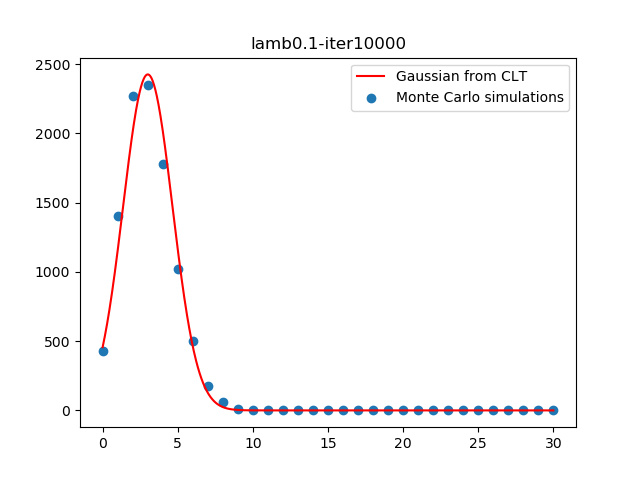
\includegraphics[width=4cm]{5_6_picture/lamb0.1-iter10000.png}
		%\caption{fig1}
		\end{minipage}%
		}%
		\subfigure[$\lambda=0.2$]{
		\begin{minipage}[t]{0.25\linewidth}
		\centering
		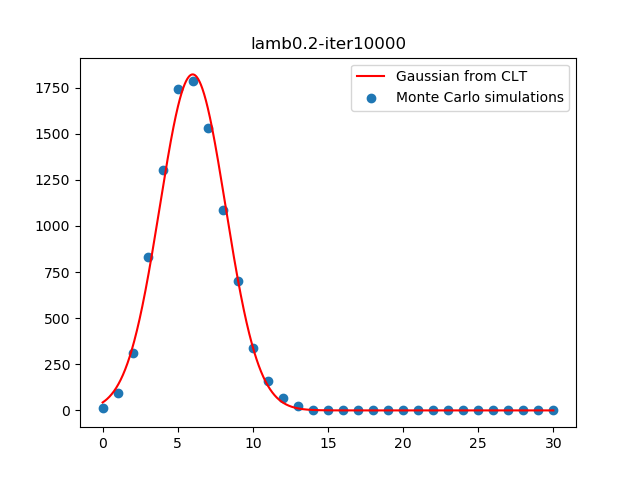
\includegraphics[width=4cm]{5_6_picture/lamb0.2-iter10000.png}
		%\caption{fig2}
		\end{minipage}%
		}%
		\subfigure[$\lambda=0.3$]{
		\begin{minipage}[t]{0.25\linewidth}
		\centering
		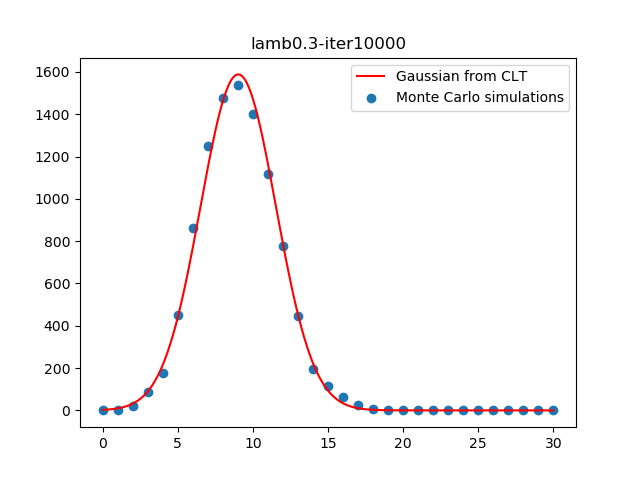
\includegraphics[width=4cm]{5_6_picture/lamb0.3-iter10000.png}
		%\caption{fig2}
		\end{minipage}%
		}%

		\subfigure[$\lambda=0.4$]{
		\begin{minipage}[t]{0.25\linewidth}
		\centering
		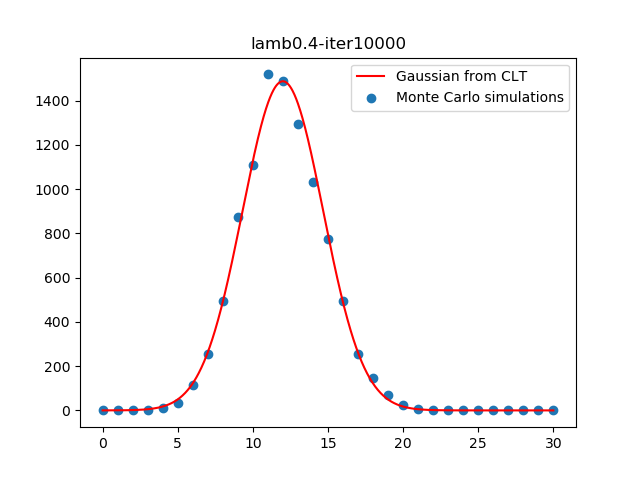
\includegraphics[width=4cm]{5_6_picture/lamb0.4-iter10000.png}
		%\caption{fig2}
		\end{minipage}
		}%
		\subfigure[$\lambda=0.5$]{
		\begin{minipage}[t]{0.25\linewidth}
		\centering
		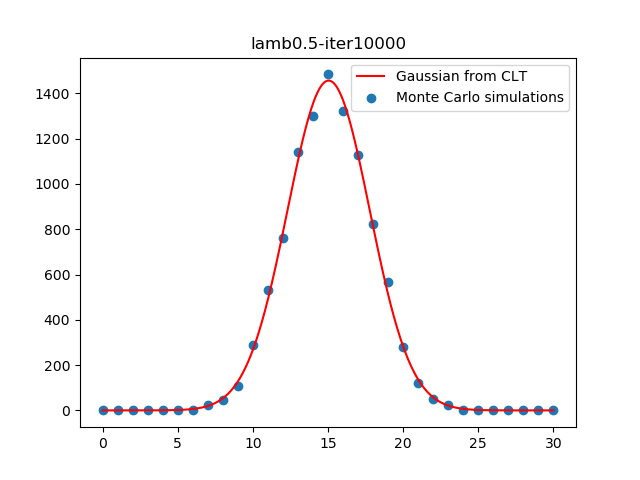
\includegraphics[width=4cm]{5_6_picture/lamb0.5-iter10000.png}
		%\caption{fig2}
		\end{minipage}
		}%
		\subfigure[$\lambda=0.6$]{
		\begin{minipage}[t]{0.25\linewidth}
		\centering
		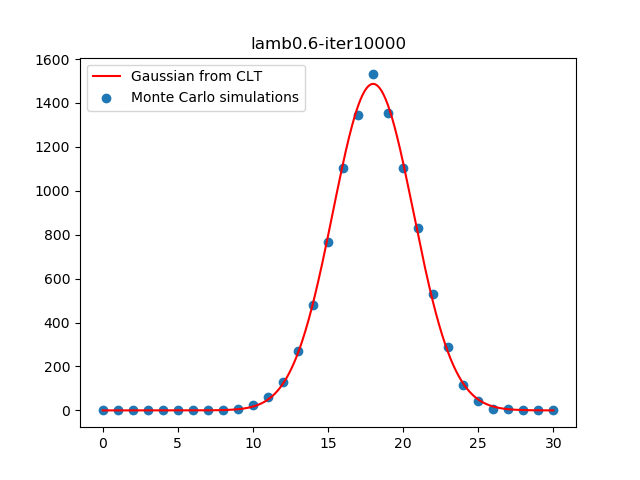
\includegraphics[width=4cm]{5_6_picture/lamb0.6-iter10000.png}
		%\caption{fig2}
		\end{minipage}%
		}%


		\subfigure[$\lambda=0.7$]{
		\begin{minipage}[t]{0.25\linewidth}
		\centering
		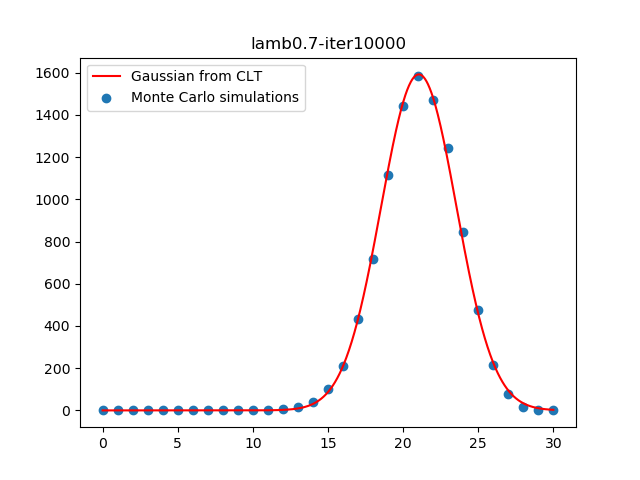
\includegraphics[width=4cm]{5_6_picture/lamb0.7-iter10000.png}
		%\caption{fig2}
		\end{minipage}%
		}%
		\subfigure[$\lambda=0.8$]{
		\begin{minipage}[t]{0.25\linewidth}
		\centering
		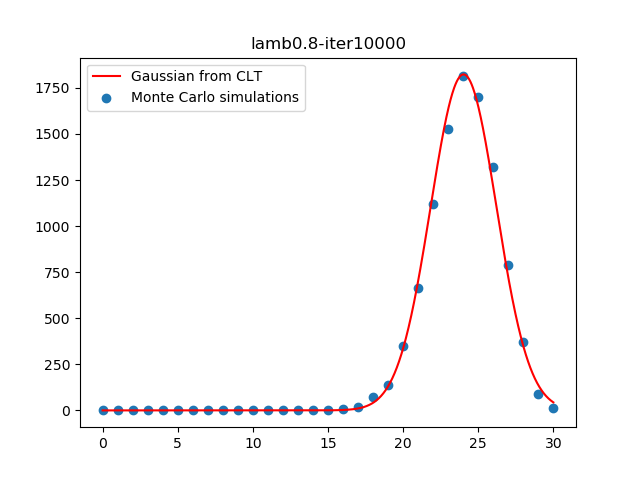
\includegraphics[width=4cm]{5_6_picture/lamb0.8-iter10000.png}
		%\caption{fig2}
		\end{minipage}%
		}%
		\subfigure[$\lambda=0.9$]{
		\begin{minipage}[t]{0.25\linewidth}
		\centering
		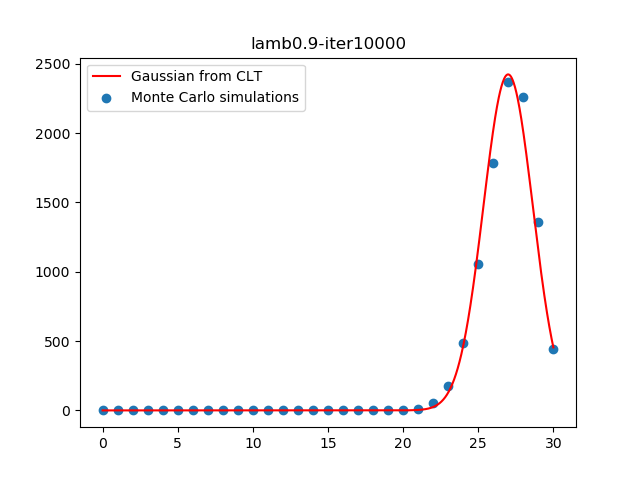
\includegraphics[width=4cm]{5_6_picture/lamb0.9-iter10000.png}
		%\caption{fig2}
		\end{minipage}%
		}%
		
		\centering
		\caption{Monte Carlo simulation and CLT results in 5.6.d}
		\label{pics56}
		\end{figure}

		Monte Carlo simulation and CLT results are in Fig. \ref{pics56}.

		Conclusion: When n becomes larger and can be regarded as continuous, the poisson distribution is similar to normal distribution.
\end {enumerate}
\end{proof}


\noindent\textbf{5.7}


(a)If X is $\sigma-$subgaussian , then $E(X)=0$,$E(X^2)\leq\sigma^2$

proof:

\begin{equation}
E(e^{\lambda X}) = \sum_{n=0}^{\infty}\frac{\lambda^n E(X^n)}{n!}=1+\lambda E(X)+\frac{\lambda^2 E(X^2)}{2}+O(\lambda^2)
\end{equation}

By definition ,

\begin{equation}
E(e^{\lambda X})\leq e^{\frac{\lambda^2 \sigma^2}{2}}=1+\frac{\lambda^2 \sigma^2}{2}+O(\lambda^2)
\end{equation}

By comparing the above two formulas and discussing the case that a approaches to 0 from above and below 0, we get the conclusion that ,

$E(X)=0$,$E(X^2)\leq\sigma^2$

(b)

If X is $\sigma-$subgaussian , then $E(X)=0$,$E(X^2)\leq\sigma^2$ .

$E(e^{c\lambda x}) = 1+\lambda E(cx)+\frac{\lambda^2 E(c^2 x^2)}{2}+O(\lambda^2)$

$\leq 1+c\lambda E(x)+\frac{\lambda^2 c^2}{2} E(x^2)+O(\lambda^2)$

$\leq 1+\frac{\lambda^2 c^2 \sigma^2}{2}+O(\lambda^2)$

$\leq e^{\frac{\lambda^2 c^2 \sigma^2}{2}}$

Hence , cX is $|c|\sigma-$subgaussian .

(c)

If $X_1$ is $\sigma_1-$subgaussian , $X_2$ is $\sigma_2-$subgaussian

then $E(X_1)=0$,$E(X_1^2)\leq\sigma_1^2$ ,$E(X_2)=0$,$E(X_2^2)\leq\sigma_2^2$

$E(e^{\lambda (x_1+x_2)}) = 1+\lambda E(x_1+x_2)+\frac{\lambda^2 E((x_1+x_2)^2)}{2}+O(\lambda^2)$

$= 1+\frac{\lambda^2}{2} Var(x_1+x_2)+O(\lambda^2)$

$= 1+\frac{\lambda^2}{2} (var(x_1)+var(x_2)+2cov(x_1,x_2))+O(\lambda^2)$

Because $x_1$, $x_2$ are independent ,

$= 1+\frac{\lambda^2}{2} (E(x_1^2) + E(x_2^2))(\lambda^2)$

$\leq 1+\frac{\lambda^2}{2} (\sigma_1^2 + \sigma_2^2)+O(\lambda^2)$

$\leq e^{\frac{\lambda^2 (\sigma_1^2 + \sigma_2^2)}{2}}$

Hence , $X_1+X_2$ is $\sqrt{\sigma_1^2 + \sigma_2^2}-$subgaussian .



\noindent\textbf{5.8}
(\textsc{Properties of subgaussian random variables (ii)})
Let $X_{i}$ be $\sigma_i$-subgaussian for $i \in\{1,2\}$ with $\sigma_i \geq 0$.
Prove that $X_{1}+X_{2}$ is $(\sigma_1 + \sigma_2)$-subgaussian.
Do \textit{not} assume independence of $X_1$ and $X_2$.

\begin{proof}
	We start straight from the definition:

	\begin{equation*}
	\begin{aligned}
	&\mathbb{E}[\exp(\lambda(X_{1}+X_{2}))]\\
	\leq &\mathbb{E}[\exp(\lambda p X_{1})]^\frac{1}{p} \mathbb{E}[\exp(\lambda q X_{2})]^\frac{1}{q}\\
	\leq &\exp(\lambda^2 p^2 \sigma_1^2 / 2)^\frac{1}{p} \exp(\lambda^2 q^2 \sigma_2^2 / 2)^\frac{1}{q}\\
	= &\exp(\frac{\lambda^2(p \sigma_1^2 + q \sigma_2^2)}{2})\\
	= &\exp(\frac{\lambda^2(\sigma_1^2 + \sigma_2^2)}{2}),
	\end{aligned}
	\end{equation*}
	where the first inequality holds according to Hölder's inequality and the last equality holds with $p = \frac{\sigma_1^2 + \sigma_2^2}{\sigma_2^2}$.
\end{proof}

\noindent\textbf{5.9}
(Properties of moment/cumulative-generating functions) Let $X$ be a real-valued random variable and let $M_X(\lambda) = \EE{\exp(\lambda X)}$ be its moment-generating function defined over $\text{dom}(M_X) \subseteq \RR$, where the expectation takes on finite values. Show that the following properties hold:
\begin{enumerate}
	\item[(a)] $M_X$ is convex, and in particular $\text{dom}(M_X)$ is an interval containing zero.
	\item[(b)] $M_X(\lambda) \ge e^{\lambda \EE{X}}$ for all $\lambda \in \text{dom}(M_X)$.
	\item[(c)] For any $\lambda$ in the interior of $\text{dom}(M_X)$, $M_X$ is infinitely many times differentiable.
	\item[(d)] Let $M^{(k)}_X(\lambda) = \frac{d^k}{d\lambda^k}M_X(\lambda)$. Then, for $\lambda$ in the interior of $\text{dom}(M_X)$, $M^{(k)(\lambda)} = \EE{X^k \exp(\lambda X)}$. 
	\item[(e)] Assuming $0$ is in the interior of $\text{dom}(M_X)$, $M^{(k)(0)} = \EE{X^k}$ (hence the name of $M_X$).
	\item[(f)] $\psi_X$ is convex (that is, $M_X$ is log-convex). 
\end{enumerate}

\begin{proof}

\begin{enumerate}
	\item[(a)] To prove $M_X$ is convex, we want to prove $\forall \alpha \in (0,1), a,b\in \text{dom}(M_X)$, there is $M_X(\alpha 
	 a + (1-\alpha)b) \le \alpha M_X(a) + (1-\alpha)M_X(b)$. 
	 \begin{align*}
	 	M_X(\alpha a + (1-\alpha)b) &= \EE{ \exp\bracket{ \alpha a + (1-\alpha)b X }} \\
	 	&\le \EE{ \alpha \exp\bracket{ a X}+ (1-\alpha)\exp\bracket{b X} } \\
	 	&= \alpha \EE{\exp\bracket{ a X}}+(1-\alpha)\EE{\exp\bracket{b X}} = \alpha M_X(a) + (1-\alpha)M_X(b)\,,
	 \end{align*}
	 where the inequality comes from the convexity of $x \to \exp(x)$.

	 To prove $\text{dom}(M_X)$ is an interval containing zero, we want to prove $M_X(0)<\infty$. It is obvious that $ M_X(0) = \EE{\exp(0\cdot X)} = \EE{\exp(0)} =1<\infty $. 
	\item[(b)] For all $\lambda \in \text{dom}M_X$, we have
	\begin{align*}
		M_X(\lambda) = \EE{ \exp(\lambda X) } \ge \exp\bracket{\EE{\lambda X}} = \exp\bracket{\lambda\EE{ X}}\,,
	\end{align*}
	where the inequality comes from the convexity of $x \to \exp(x)$.
	\item[(c)] TBD
	\item[(d)] $M^{(1)}_X(\lambda) = \frac{d}{d\lambda} \EE{\exp(\lambda X)}= \EE{\frac{d}{d\lambda} \exp(\lambda X)} = \EE{X \exp(\lambda X)}$. 
	Recursively, we have $M^{(k)}_X(\lambda) = \EE{X^k \exp(\lambda X)}$. 
	\item[(e)] According to the result of (d), we have $M^{(k)}_X(0) = \EE{X^k \exp(0\cdot X)} = \EE{X^k}$.
	\item[(f)] To prove $\psi_X$ is convex, we want to prove $\forall \alpha \in (0,1), a,b\in \text{dom}(\psi_X)$, there is $\psi_X(\alpha a + (1-\alpha)b) \le \alpha \psi_X(a) + (1-\alpha)\psi_X(b)$.
	\begin{align*}
		\psi_X(\alpha a + (1-\alpha)b) &= \log M_X( \alpha a + (1-\alpha)b ) \\
		&= \log \EE{\exp\bracket{ \alpha a + (1-\alpha)b}X} \\
		&= \log \EE{\exp\bracket{ \alpha aX } \exp((1-\alpha)bX)} \\
		&= \log \EE{\bracket{\exp\bracket{ aX }}^{\alpha} \bracket{\exp(bX)}^{(1-\alpha)}}\\
		&\le  \log \bracket{ \EE{\exp\bracket{ aX }}^{\alpha } \EE{\exp(bX)}^{(1-\alpha)} } \\
		&= \alpha \log \EE{ \exp\bracket{ aX } } + (1-\alpha) \EE{\exp(bX)} = \alpha \psi_X(a) + (1-\alpha)\psi_X(b) \,,
	\end{align*}
	where the inequality comes from the Hölder's inequality. 
\end{enumerate}

\end{proof}


\noindent\textbf{5.10} (Large deviation theory) Let $X,X_1,X_2,...,X_n$ be a sequence of independent and identically distributed random variables with zero mean and moment-generating function $M_X$ with $dom(M_X)=\RR.$ Let$\hat{\mu}_n=\frac{1}{n}\sum_{t=1}^nX_t$.
\begin{enumerate}
    \item[(a)]Show that for any $\epsilon>0$,
        \begin{align}
            \frac{1}{n}\log\PP{\hat{\mu}_n\geq\epsilon}\leq -\psi_X^{\ast}(\epsilon)=-\underset{\lambda}{\sup}(\lambda\epsilon-\log M_X(\lambda))
        \end{align}
    \item[(b)]Show that when X is a Rademacher variable$(\PP{X=1}=\PP{X=-1}=\frac{1}{2})$,$\psi_X^{\ast}(\epsilon)=\frac{1+\epsilon}{2}\log(1+\epsilon)+\frac{1-\epsilon}{2}\log(1-\epsilon)$when$\abs{\epsilon}\le 1$ and $\psi_X^{\ast}(\epsilon)=+\infty$,otherwise.
\end{enumerate}

\begin{proof}
\begin{enumerate}
	\item[(a)] For all $\lambda\in domM_X$,we have 
	    \begin{align*}
	        \frac{1}{n}\log\PP{\hat{\mu}_n\geq\epsilon}&=\frac{1}{n}\log\PP{\exp{(\lambda n\hat{\mu}_n)}\geq\exp{(\lambda n \epsilon)}}\\
	        &\leq \frac{1}{n}\log(\EE{\exp{(\lambda n\hat{\mu}_n)}}\exp{(-\lambda n \epsilon)})\\
	        &=\frac{1}{n}\log(\prod_{t=1}^n\EE{\exp{(\lambda X_t)}}\exp{(-\lambda n \epsilon)})\\
	        &=\frac{1}{n}\log(\EE{\exp{(\lambda X)}}^n\exp{(-\lambda n \epsilon)})\\
	        &=\log(\EE{\exp{(\lambda X)}}\exp{(-\lambda\epsilon)})\\
	        &=-(\lambda\epsilon-\log M_X(\lambda))
	    \end{align*}
        Since it holds for all $\lambda\in domM_X$,we can imply
        \begin{align*}
            \frac{1}{n}\log\PP{\hat{\mu}_n\geq\epsilon}\leq -\psi_X^{\ast}(\epsilon)=-\underset{\lambda}{\sup}(\lambda\epsilon-\log M_X(\lambda))
        \end{align*}

	\item[(b)] By definition, $\psi_{X}(\lambda)=\log(\frac{1}{2}(\exp (-\lambda)+\exp (\lambda)))= \log(\cosh (\lambda))$, where $\cosh(\cdot)$ is the hyperbolic cosine function.
	To find the maximum of $f(\lambda) = \lambda \varepsilon - \psi_{X}(\lambda)$, we have $f^\prime(\lambda) = \varepsilon - \tanh(\lambda)$, where $\tanh(\lambda) = \frac{\exp(\lambda) - \exp(-\lambda)}{\exp(\lambda) + \exp(-\lambda)}$ is the hyperbolic tangent function.
	Since $\tanh(\lambda) \in[-1,1]$, $\sup _{\lambda} f(\lambda)=+\infty$ when $|\varepsilon|>1$.
	Otherwise, we have
	\begin{equation*}
		\begin{aligned}
			\psi_{X}^{*}(\varepsilon)
			&=f\left(\tanh ^{-1}(\varepsilon)\right)\\
			&=\tanh ^{-1}(\varepsilon) \varepsilon-\log \cosh \left(\tanh ^{-1}(\varepsilon)\right)\\
			&=\frac{\varepsilon}{2} \log \left(\frac{1+\varepsilon}{1-\varepsilon}\right)+\frac{1}{2} \log \left(1-\varepsilon^{2}\right)\\
			&=\frac{1+\varepsilon}{2} \log (1+\varepsilon)+\frac{1-\varepsilon}{2} \log (1-\varepsilon),
		\end{aligned}
	\end{equation*}
	where the second equality holds as $\tanh ^{-1}(\varepsilon)=\frac{1}{2} \log \left(\frac{1+\varepsilon}{1-\varepsilon}\right)$.
\end{enumerate}
\end{proof}


\noindent\textbf{5.11} (Hoeffding's lemma) Suppose that $X$ is zero mean and $X \in [a,b]$ almost surely for constants $a <b$.
\begin{enumerate}
	\item[(a)]Show that $X$ is $(b-a)/2$-subgaussian.
	\item[(b)]Prove Hoeffding's inequality (Lemma \ref{lem:hoeffding}).
\end{enumerate}
\begin{lemma}[Hoeffding's inequality]\label{lem:hoeffding}
	For a zero-mean random variable $X$ such that $X \in [a,b]$ almost surely for real values $a <b$, then $M_X(\lambda) \le \exp(\lambda^2 (b-a)^2 / 8)$. Applying the Cramér–Chernoff method shows that if $X_1,X_2,\ldots,X_n$ are independent and $X_t \in [a_t,b_t]$ almost surely with $a_t < b_t$ for all $t$. Then, 
	\begin{align}
		\PP{\frac{1}{n} \sum_{t=1}^n \bracket{X_t - \EE{X_t}} \ge \varepsilon } \le \exp\bracket{ \frac{-2n^2\varepsilon^2}{\sum_{t=1}^n (b_t-a_t)^2 } }\,.
	\end{align}
\end{lemma}

\begin{proof}
\begin{enumerate}
	\item[(a)]To show $X$ is $(b-a)/2$-subgaussian, we want to prove $\forall \lambda \in \RR, \EE{\exp(\lambda X)} \le \exp\bracket{ \frac{\lambda^2 (b-a^2)}{8} }$.

	According to the convexity of $x \to \exp(x)$ and Jensen's inequality, we have $\forall X \in [a,b]$,
	\begin{align*}
		\exp(\lambda X) = \exp\bracket{ \frac{b-X}{b-a}\lambda a + \frac{X-a}{b-a}\lambda b } \le \frac{b-X}{b-a}\exp(\lambda a)+ \frac{X-a}{b-a}\exp(\lambda b)\,.
	\end{align*}
	Thus, 
	\begin{align*}
		\EE{\exp(\lambda X)} &\le \frac{b-\EE{X}}{b-a}\exp(\lambda a)+ \frac{\EE{X}-a}{b-a}\exp(\lambda b) \\
		&= \frac{b}{b-a}\exp(\lambda a)+ \frac{-a}{b-a}\exp(\lambda b)\\
		&= (1-\theta)\exp(\lambda a)+\theta \exp(\lambda b) ~~~\bracket{\text{By letting $\theta = \frac{-a}{b-a}$}} \\
		&= \exp(\lambda a) \bracket{1-\theta+\theta \exp(\lambda b - \lambda a)} \\
		&= \exp(-\lambda(b-a)\theta) \bracket{ 1-\theta+\theta \exp(\lambda b - \lambda a) } ~~~\bracket{\text{By representing $a$ using $\theta$}}\\
		&= \exp\bracket{-\theta u + \log(1-\theta+\theta\exp(u))} ~~~\bracket{\text{By letting $u=\lambda(b-a)$} } \\
		&= \exp(\phi(u)), ~~~\text{where}~~ \phi(u)=-\theta u + \log(1-\theta+\theta\exp(u))\,.
	\end{align*}
	We next want to find the upper bound for $\exp(\phi(u))$. According to the Taylor's theorem with mean-values forms of the remainder, we have 
	\begin{align*}
		\phi(u) &= \phi(0) + u\phi'(0) + \frac{1}{2}u^2 \phi''(v),~~~~\text{where}~v \in (0,u)\\
		&= \frac{1}{2}u^2 \phi''(v) ~~~\bracket{\text{Since $\phi(0) = \phi'(0) = 0$}}\\
		&= \frac{1}{2}u^2 \cdot \frac{\theta \exp(v)}{1-\theta+\theta \exp(v)}\bracket{1-\frac{\theta \exp(v)}{1-\theta+\theta \exp(v)}} \\
		&\le \frac{1}{2}u^2 \cdot \frac{1}{4} =\frac{1}{8}u^2 = \frac{\lambda^2 (b-a)^2}{8}\,.
	\end{align*}
	Above all, we have proved that $\forall \lambda \in \RR, \EE{\exp(\lambda X)} \le \exp(\phi(u)) \le \exp\bracket{\frac{\lambda^2 (b-a)^2}{8}}$. 


	\item[(b)]  We only give the upper tail of the Hoeffding's Inequality using the Hoeffding's Lemma since the lower tail has a similar proof. Applying the Hoeffding' Lemma and the Chernoff bound technique immediately
	shows that
	\begin{align*}
		\mathbb{P}\left(\frac{1}{n}\sum^n_{t=1}(X_t -\mathbb{E}[X_t])\geq\epsilon\right)&=\mathbb{P}\left(\sum^n_{t=1}(X_t-\mathbb{E}[X_t])\geq n\epsilon \right)\\
		&\leq\mathbb{E}\left[\exp\left(\lambda\sum^n_{t=1}(X_t-\mathbb{E}[X_t]) \right) \right]e^{-\lambda n\epsilon}\\
		&=\left(\Pi^n_{t=1}\mathbb{E}[\exp\left(\lambda(X_t-\mathbb{E}[X_t])\right)] \right)e^{-\lambda n\epsilon}\\
		&\leq\left(\Pi^n_{t=1}e^{\frac{\lambda^2(b_t-a_t)^2}{8}} \right)e^{-\lambda n\epsilon}\,,
	\end{align*}
	where $\lambda\geq0$. Minimizing the RHS of the above inequality over $\lambda$ shows that
	\begin{align*}
		\mathbb{P}\left(\frac{1}{n}\sum^n_{t=1}(X_t -\mathbb{E}[X_t])\geq\epsilon\right)\leq \min_{\lambda\geq0}\left(\Pi^n_{t=1}e^{\frac{\lambda^2(b_t-a_t)^2}{8}} \right)e^{-\lambda n\epsilon} =\exp\left(\frac{-2n^2\epsilon^2}{\sum^n_{t=1}(b_t-a_t)^2}\right)\,.
	\end{align*}
\end{enumerate}
\end{proof}



% (a)
% \begin{equation}
% E(e^{\lambda X}) = 1+\lambda E(X)+\frac{\lambda^2 E(X^2)}{2}+O(\lambda^2) =1+\frac{\lambda^2 E(X^2)}{2}+O(\lambda^2)
% \end{equation}

% If the conclusion is true, then the above formula satisfies

% $\leq 1+\frac{\lambda^2}{2}(\frac{(b-a)^2}{4})+O(\lambda^2)$

% So just prove:

% $E(x^2)\leq (\frac{b-a}{2})^2$

% $E(x^2)=var(x)=E(x-\bar{x})^2$

% However,$(x-\bar{x})^2\leq(\frac{b-a}{2})^2$ . The conclusion is proved.

% (b)

% The proof of Hoeffding's Inequality:

% Let $X_i = Z_i - E(Z_i)$ , $\bar{X} = \frac{1}{m}\sum_{i=1}^{m}X_i$

% By Markov inequality , for all $\lambda >0$ , $\varepsilon > 0$,

% $P(\bar{X}\geq\varepsilon) = P(e^{\lambda \bar{X}} \geq e^{\lambda\varepsilon}) \leq \frac{E(e^{\lambda \bar{X}})}{e^{\lambda\varepsilon}}$

% $Z_1$,$\cdots$,$Z_m$ iid.r.v.

% So,$E(e^{\lambda \bar{X}}) = \prod_{i=1}^{m} E(e^{\frac{\lambda X_i}{m}})$

% By Hoeffding's lamma,

% $ E(e^{\frac{\lambda X_i}{m}}) \leq e^{\frac{\lambda^2(b-a)^2}{8m^2}}$

% So , $P(\bar{X}\geq\varepsilon) \leq e^{-\lambda\varepsilon}\prod_{i=1}^{m} E(e^{\frac{\lambda X_i}{m}})$

% $\leq e^{-\lambda\varepsilon}e^{\frac{\lambda^2(b-a)^2}{8m}}$

% $\leq e^{-\lambda\varepsilon+\frac{\lambda^2(b-a)^2}{8m}}$

% Let $\lambda = \frac{4m\varepsilon}{(b-a)^2}$ , then $P(\bar{X}\geq \varepsilon) \leq e^{\frac{-2m\varepsilon^2}{(b-a)^2}}$

% Similarly, we can prove the other side of the inequality.


\noindent \textbf{5.16}
By assumption $Pr(X_t\leq x)\leq x$, which means that for$\lambda <1$,
\begin{align}
\mathbb{E}\left[exp(\lambda log(\frac{1}{x_t}))\right] = \int_0^\infty P(exp(\lambda log(\frac{1}{x_t}))\geq x)dx = 1 +\int_1^\infty P(X_t \leq x^{-\frac{1}{\lambda}})dx
\end{align}
Applying the Cramer-Chernoff method,
$$P\left(\sum_{t=1}^n log(\frac{1}{X_t}) \geq \epsilon\right) = P\left(exp(\lambda \sum_{t=1}^n log(\frac{1}{X_t})) \geq exp(\lambda \epsilon) \right) \leq \left(\frac{1}{1-\lambda}\right)^n exp (-\lambda \epsilon)$$
choosing $\lambda  = \frac{\epsilon-n}{\epsilon}$ completes the claim.



\noindent \textbf{5.18} (\textsc{Expectation of maximum})
Let $X_{1}, \ldots, X_{n}$ be a sequence of $\sigma$-subgaussian random variables
(possibly dependent) and $Z=\max _{t \in[n]} X_{t}$. Prove that

\begin{itemize}
	\item[(a)] $\mathbb{E}[Z] \leq \sqrt{2 \sigma^{2} \log (n)}$.
	\item[(b)] $\mathbb{P}\left(Z \geq \sqrt{2 \sigma^{2} \log (n / \delta)}\right) \leq \delta \text { for any } \delta \in(0,1)$.
\end{itemize}

\begin{proof}
	\begin{itemize}
		\item[(a)] Let $\lambda >0$.
		Then,
		\begin{equation*}
			\exp(\lambda \mathbb{E}[Z]) \leq \mathbb{E}[\exp(\lambda Z)] \leq \sum_{t=1}^n \mathbb{E}[\exp(\lambda X_t)] \leq n \exp(\frac{\lambda^2 \sigma^2}{2}).
		\end{equation*}
		
		Rearranging shows that
		\begin{equation*}
			\mathbb{E}(Z) \leq \frac{log(n)}{\lambda} + \frac{\lambda \sigma^2}{2}.
		\end{equation*}
	
		Choosing $\lambda = \frac{1}{\sigma} \sqrt{2log(n)}$ shows that $\mathbb{E}(Z) \leq \sqrt{2\sigma^2 log(n)}$
		
		\item[(b)] First notice that
		\begin{equation*}
			\begin{aligned}
				\mathbb{P}\left(Z \geq \sqrt{2 \sigma^{2} \log (n / \delta)}\right)
				&= \mathbb{P}\left(\exists i: X_i \geq \sqrt{2 \sigma^{2} \log (n / \delta)}\right)\\
				&\leq \sum_{i=1}^n \mathbb{P}\left(X_i \geq \sqrt{2 \sigma^{2} \log (n / \delta)}\right),
			\end{aligned}
		\end{equation*} 
		which is given directly by a union bound.

		Then, according to Theorem 5.3, we have $\mathbb{P}\left(X_i \geq \sqrt{2 \sigma^{2} \log (n / \delta)}\right)
		\leq \frac{\delta}{n}$ to complete the proof.
	\end{itemize}
\end{proof}

\input{Ch6}
\input{Ch7}
\input{Ch8}
\input{Ch9}
\input{Ch10}
\input{Ch11}
\input{Ch18}
\input{Ch28}
\chapter*{Chapter 38 Markov Decision Processes}
\label{sec:thirty_eighth}

\noindent\textbf{38.5} (Diameter lower bound) Let $M = (S, A, P, r)$ be any MDP. Show that $D(M) \ge\log_A(S) - 3$.

\begin{proof}
Denote by $d^∗(s, s' )$ the minimum expected time it takes to reach state $s'$ when starting from
state $s$. The definition of $d^∗$ can be extended to arbitrary initial distributions $\mu_0$ over states and sets $U \subset S$ of target states: $d^∗(\mu_0,U) = \sum_s \mu_0(s) \sum_{s'\in U}d^*(s, s')$. Prove by induction on the size of $U$ that
\begin{align*}    
    d^*(\mu_0,U) \ge \min\set{ \sum_{k\ge 0}k n_k\big| 0\le n_k \le A^k, k\ge0,\sum_{k\ge 0} n_k = |U|} \,.
\end{align*}

Note that the minimum of $d^*(s,s')$ is attained when $n_k$ is maximised. That is, $n_0=A^0, n_1 = A^1,\cdots n_{m-1} = A^{m-1}, n_m = |U|-\sum_{k=0}^{m-1}A^k \leq A^m$. We futher have that
\begin{align*}
    &|U|\ge \sum_{k=0}^{m-1}A^k\\
    &|U| \leq \sum_{k=1}^{m-1}A^k + A^m \leq 2A^{m} \rightarrow m\ge \log_A\frac{|U|}{2}\,.
\end{align*}

Thus we can obtain the lower bound of $D(m)$ by letting $S=U$:
\begin{align*}
    d^*(\mu_0,U) &= \sum_{k=0}^{m-1}kA^k + n_m m\\
    &=\sum_{k=0}^{m-1}kA^k + m\left(|U|-\sum_{k=0}^{m-1}A^k\right)\\
    &= m|U| + \sum_{k=0}^{m-1}(k-m) A^k\\
    &=m|U| + \frac{m}{A-1} - \frac{A(A^m-1)}{(A-1)(A-1)}\\
    &\ge m|U| - \frac{A}{A-1} |U|\\
    &\ge |U|(m-2)\\
    &\ge |U|\left(\log_A|U|-3\right) \,.
\end{align*}
\end{proof}

\end{document}